\chapter{Data Link Layer}

\section{Preamble}
\subsection{Device Terminology}
\begin{center}
    \begin{tabular}{l l l}
        \textbf{Device}                 & \textbf{Layer} & \textbf{Description}                                                  \\
        Repeaters/Hubs                  & Physical       & Boost signals by repeating all received.                              \\
        Switches/Bridges                & Data Link      & Make interconnection decisions based on \keyword{MAC Addresses}.      \\
        Multi-Protocol Routers/Gateways & Data Link      & Forwards (and possibly fragment) packets. Use \keyword{IP} addresses. \\
    \end{tabular}
\end{center}
\keyword{Transport Layer} and \keyword{Application layer} \keyword{Gateways} also exist.
\\
\\ Routers act as \keyword{Gateways} to connect \keyword{IP}-based networks.

\subsection{Network Types}
Network Types ordered by size (small $\to$ large).
\begin{center}
    \begin{tabular}{l l}
        \keyword{PAN} & Personal Area Network     \\
        \keyword{LAN} & Local Area Network        \\
        \keyword{MAN} & Metropolitan Area Network \\
        \keyword{WAN} & Wide Area Network         \\
    \end{tabular}
\end{center}

\subsection{Network Topologies}
\begin{center}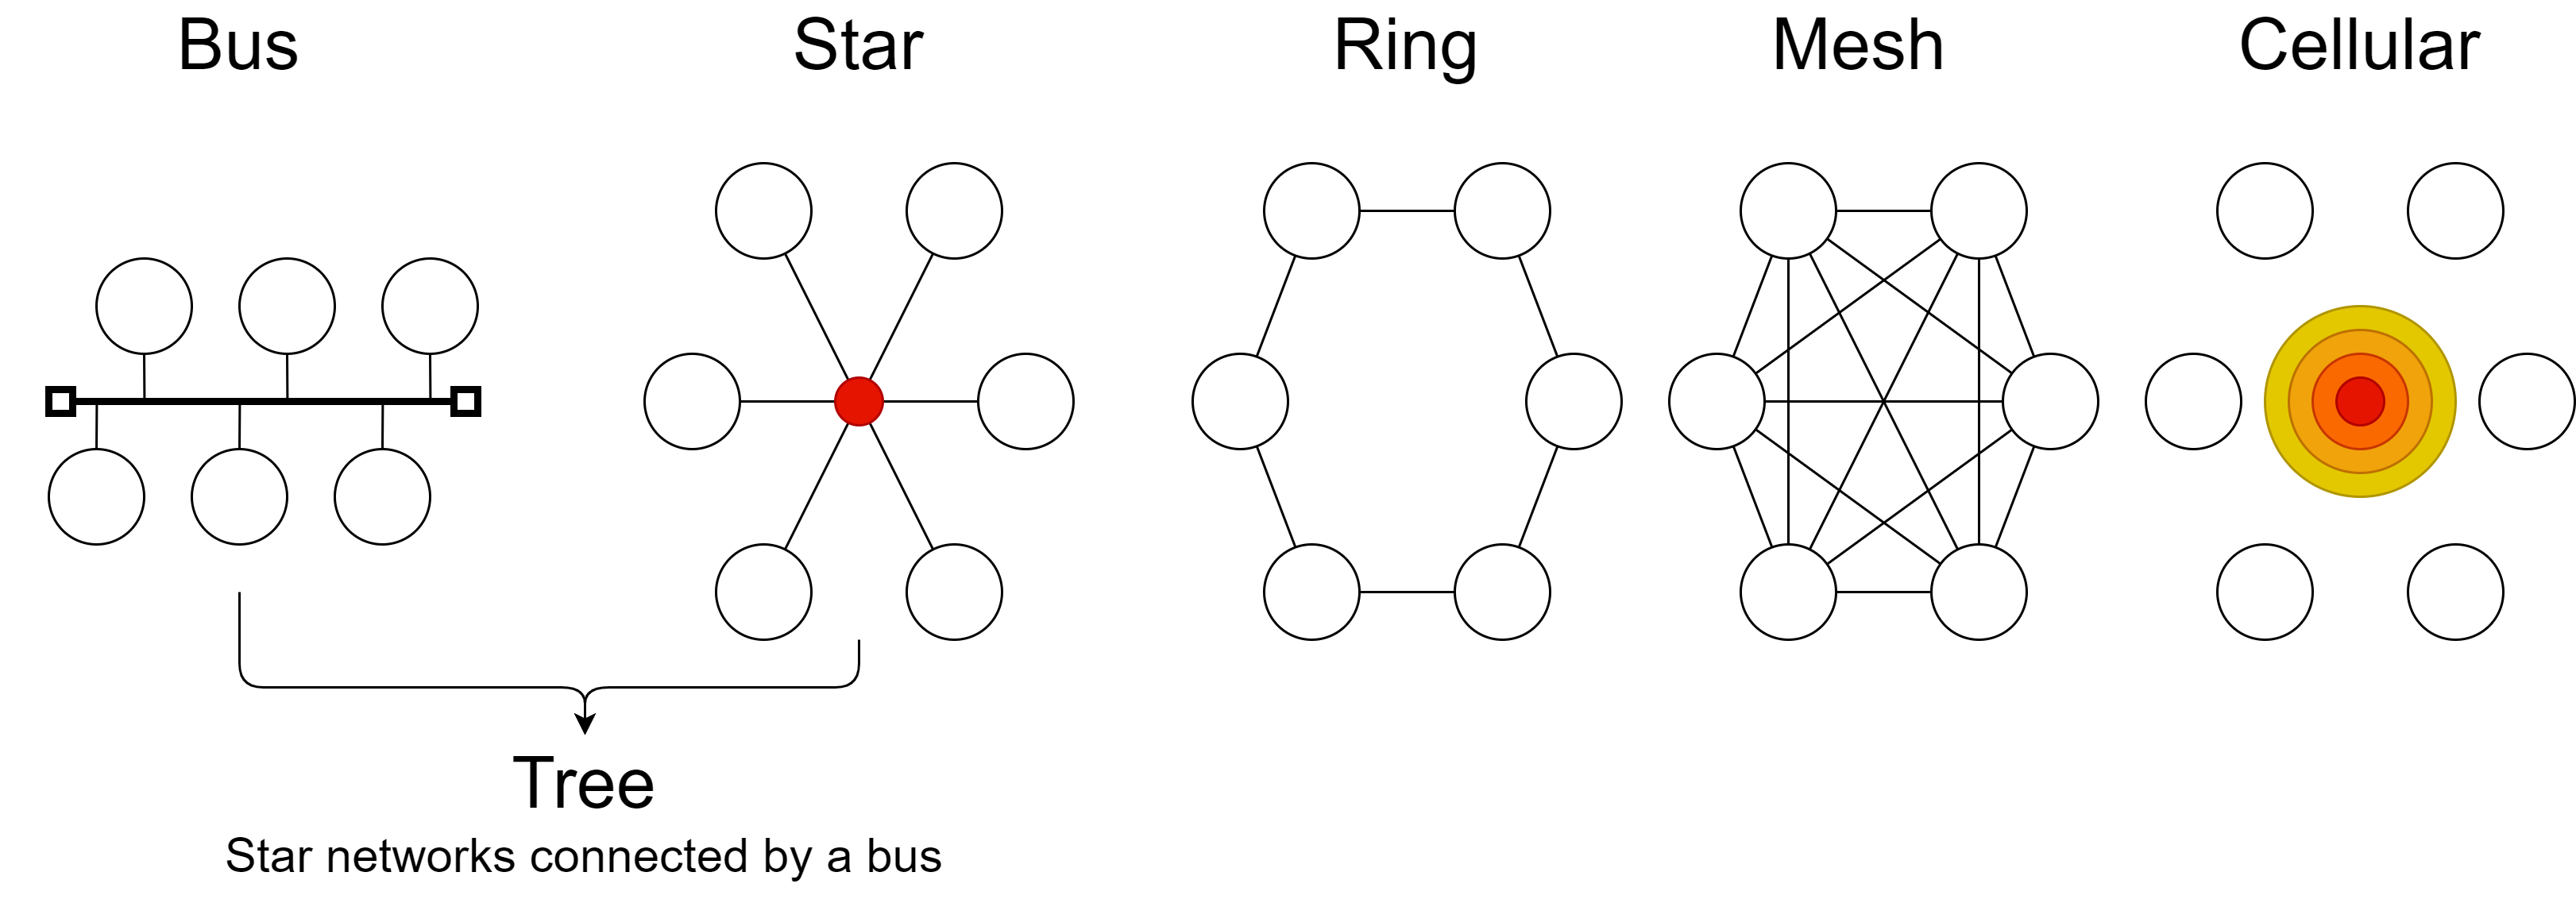
\includegraphics[width=0.9\textwidth]{data_link_layer/images/network topologies}\end{center}

\subsection{Data Link Layer Protocols}
\begin{center}
    \begin{tabular}{l l l l l}
        802.3  & Ethernet              & LAN        & 1-persistent CSMA/CD & Star/Bus  \\
        802.4  & Token Bus             & LAN        & Token Passing        & Bus/Tree  \\
        802.5  & Token Ring            & LAN        & Token Passing        & Ring      \\
        802.6  & DQDB                  & MAN        & Distributed Queue    & Bus       \\
        802.9  & isoEthernet           & LAN        & Ethernet + ISDN      & Star/Mesh \\
        802.11 & WiFi                  & LAN        & CSMA/CA              & Cellular  \\
        802.12 & 100BaseVG             & LAN        & Handshaking from hub & Star/Tree \\
        802.15 & Bluetooth             & PAN        & Adaptive FHSS        & Cellular  \\
        802.16 & WiMAX                 & MAN        & Connection oriented  & Cellular  \\
        802.17 & Resilient Packet Ring & LAN to WAN & Distributed Queue    & Ring      \\
    \end{tabular}
\end{center}

\section{Ethernet}
\termdef{Ethernet}{
    A \keyword{Data-Link Layer} protocol used for \keyword{LAN}/\keyword{MAN}/\keyword{WAN} communications.
    \compitem{
        \item \href{http://decnet.ipv7.net/docs/dundas/aa-k759a-tk.pdf}{Specification} created in 1980.
        \item Became IEEE Standard $802.3$ in 1983.
        \item Originally coaxial cable (\keyword{10BASE5}), $\approx 2.94 Mbps$
        \item Currently fibre optic, twinaxial (two coaxial) cable $\approx 100 Gbps$.
    }
}

\subsection{Ethernet Cables}
\twosplit{
    \begin{center}
        \begin{tabular}{l  l l}
            \keyword{UTP}  & Unshielded Twisted Pair         \\
            \keyword{STP}  & Shielded/Screened Twisted Pair  \\
            \keyword{FTP}  & Foiled Twisted Pair             \\
            \keyword{SFTP} & Shielded \& Foiled Twisted Pair \\
        \end{tabular}
    \end{center}
}{
    The most popular is \keyword{UTP} of which the most used version is \keyword{Cat5e}.
    \\
    \\ \keyword{Cate6a},\keyword{Cat7a} exist and \keyword{Cat8} in development.
}
Cables use shielding to protect against \keyword{ElectroMagnetic Interference} (\keyword{EMI}) (e.g crosstalk between the wires) causing errors in data transmission.

\sidenote{Lantenna Attack}{
    Sheilding can also help to reduce electromagnetic leakage from ethernet cables that can be sniffed and exploited.
    \\
    \\ A team from Ben-Gurion Univeristy have demonstrated this by attacking their own basic air-gapped networks. Their paper can be read \href{https://arxiv.org/pdf/2110.00104.pdf}{here}.
}
\begin{center}
    \begin{tabular}{l l l l l}
        \textbf{Cable Code} & \textbf{Name}         & \textbf{Cable}            & \textbf{Max Length} & \textbf{Topology} \\
        10Base5             & Thick Ethernet        & 1/2 inch coaxial cable    & 500                 & Bus               \\
        10Base2             & Thin Ethernet         & 75-Ohm coaxial cable      & 180                 & Bus               \\
        10BaseT             & Twisted Pair Ethernet & Category 3 UTP            & 100                 & Star              \\
        100Base-TX          & Fast Ethernet         & Category 5 UTP            & 100                 & Star              \\
        100Base-FX          & Fast Ethernet         & Fiber Optic               & 185                 & Star              \\
        1000Base-T          & Gigabit Ethernet      & Category 6 UTP (4 pairs)  & 100                 & Star              \\
        10GBase-T           & 10 Gigabit Ethernet   & Category 6a UTP (4 pairs) & 100                 & Star              \\
    \end{tabular}
\end{center}

\subsection{Ethernet Pinouts}
There are two main pinout wirings, the only differences are the yellow and green cables are in swapped positions:
\\ \twosplit{
    \begin{center}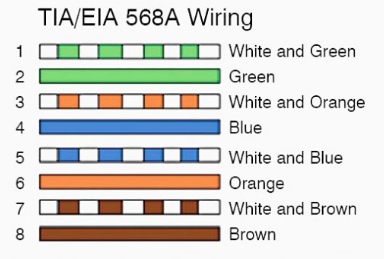
\includegraphics[width=0.9\textwidth]{data_link_layer/images/Pinouts/568A}\end{center}
}{
    \begin{center}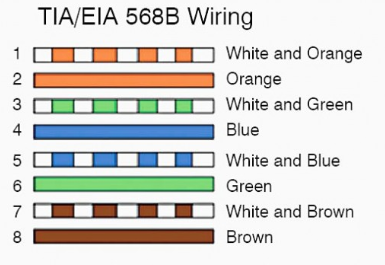
\includegraphics[width=0.9\textwidth]{data_link_layer/images/Pinouts/568B}\end{center}
}

\subsubsection{Straight Through}
\twosplit{
    \begin{center}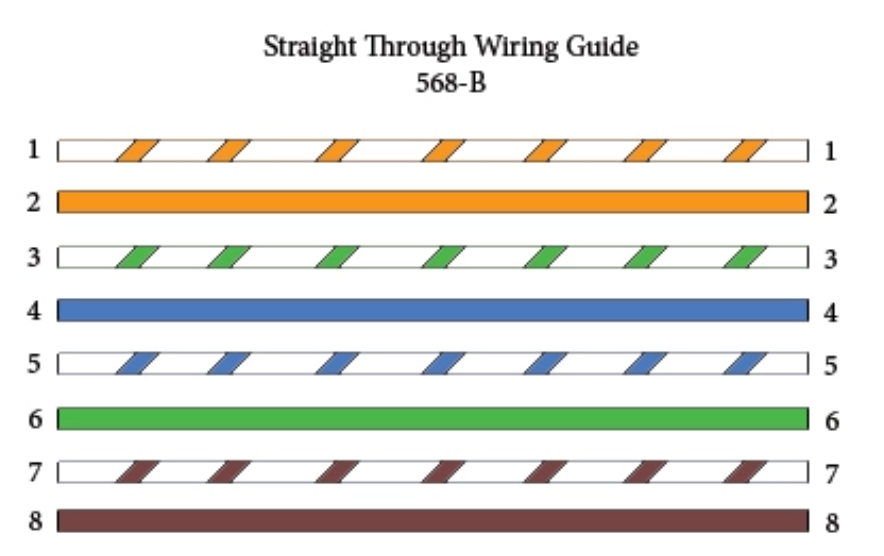
\includegraphics[width=0.9\textwidth]{data_link_layer/images/Pinouts/straight through}\end{center}
}{
    Communication between different OSI layers (e.g switch $\to$ router).
    \\
    \\ This is also called the \keyword{Media/Medium Dependent Interface} (\keyword{MDI})
}

\subsubsection{Crossover}
\twosplit{
    \begin{center}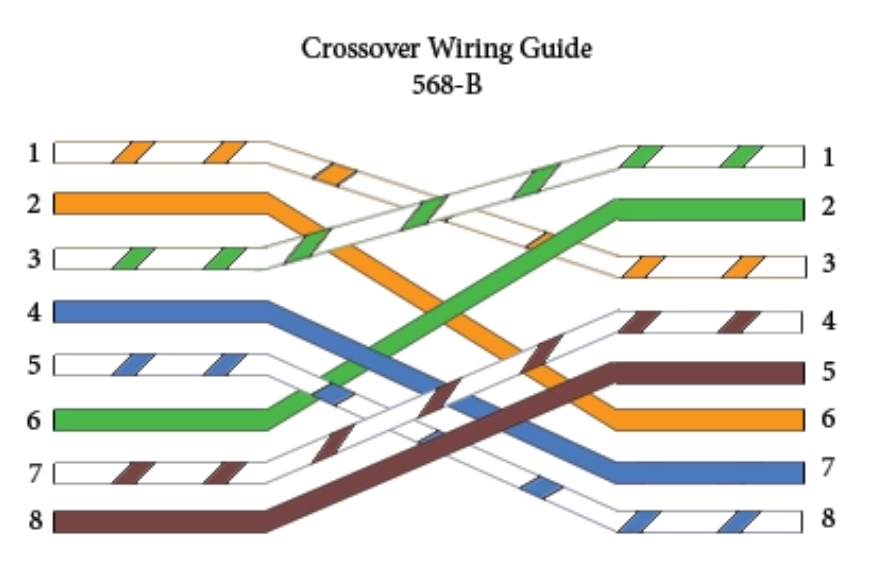
\includegraphics[width=0.9\textwidth]{data_link_layer/images/Pinouts/crossover}\end{center}
}{
    Communication between devices on the same OSI layer (e.g switch $\to$ switch).
    \\
    \\ This is also called the \keyword{Media/Medium Dependent Interface with Crossover} (\keyword{MDIX})
}
\twosplit{
    \begin{center}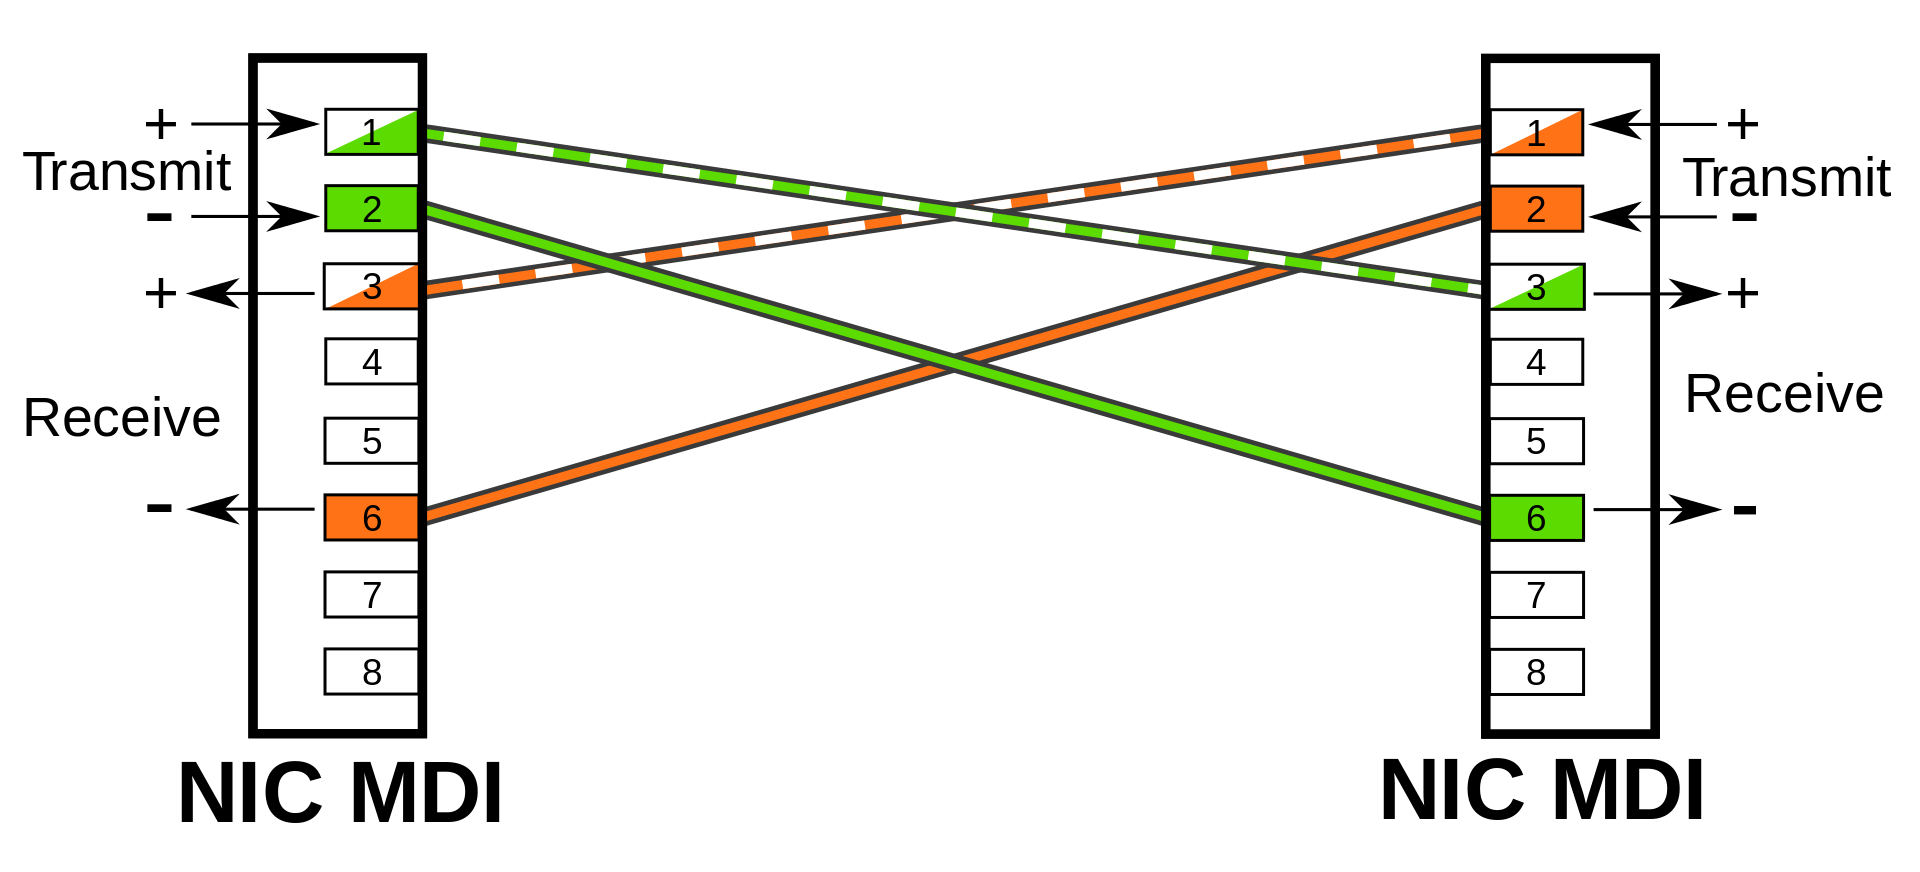
\includegraphics[width=0.9\textwidth]{data_link_layer/images/Pinouts/crossover explained}\end{center}
}{
    The crossover connects the transmit on one side, to the receive on the other side and vice-versa. As the devices are the same OSI layer, they can communicate back and forth through this.
}

\subsubsection{Rollover}
\twosplit{
    \begin{center}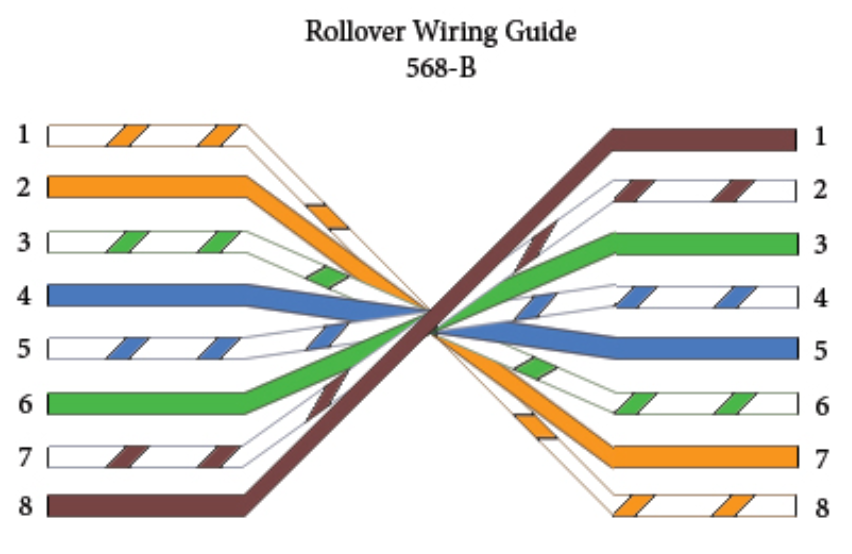
\includegraphics[width=0.9\textwidth]{data_link_layer/images/Pinouts/rollover}\end{center}
}{
    Used to directly tap into a network device (e.g a console to debug a router setup issue)
}

\example{Connect Computer to Router}{
    \begin{center}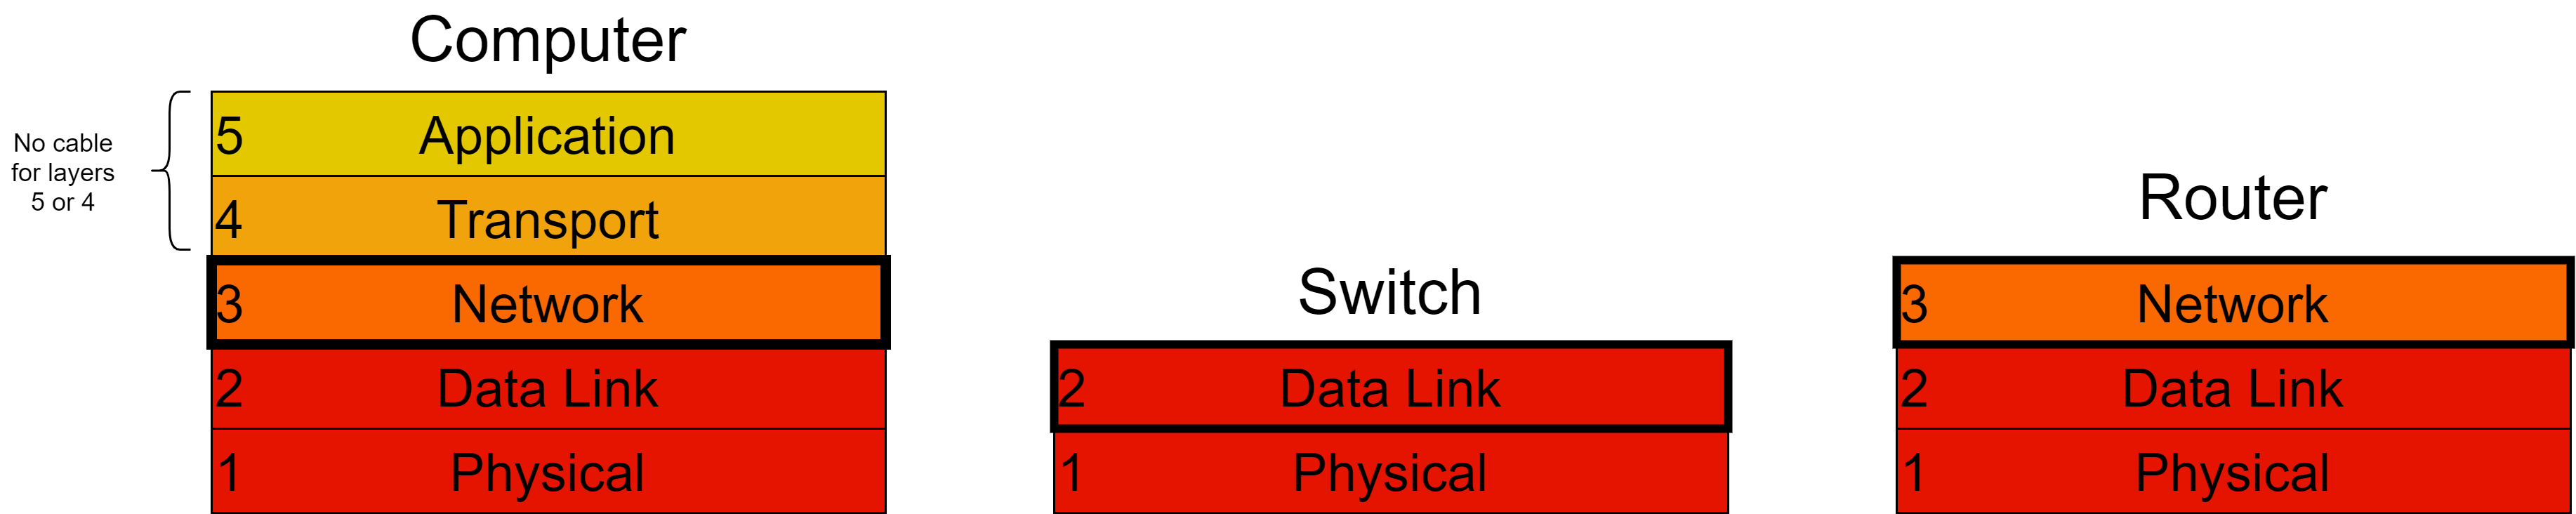
\includegraphics[width=0.9\textwidth]{data_link_layer/images/computer to router example}\end{center}
    When we connect to a router, we will be connecting to a switch (with a router attached).
    \\
    \\ We consider the computer as \keyword{Network Layer} as that is the highest we can directly connect, and the switch as \keyword{Data Link Layer}. Hence a straight-through connection is used as they are different \keyword{OSI Layers}.
}

\subsection{Ethernet Frame}
\termdef{Octet}{
    A byte/$8$ bits. It is used as an unambiguous term as on older machines the definition of a byte was hardware dependent (e.g like the term word). The \href{https://en.wikipedia.org/wiki/Byte}{wikipedia page for byte} contains many interesting sources with examples ranging from $1$ bit to $48$ bit bytes).
    \\
    \\ Nowadays a byte is always $8$ bits, so can be used interchangably with \keyword{octet}
}
\begin{center}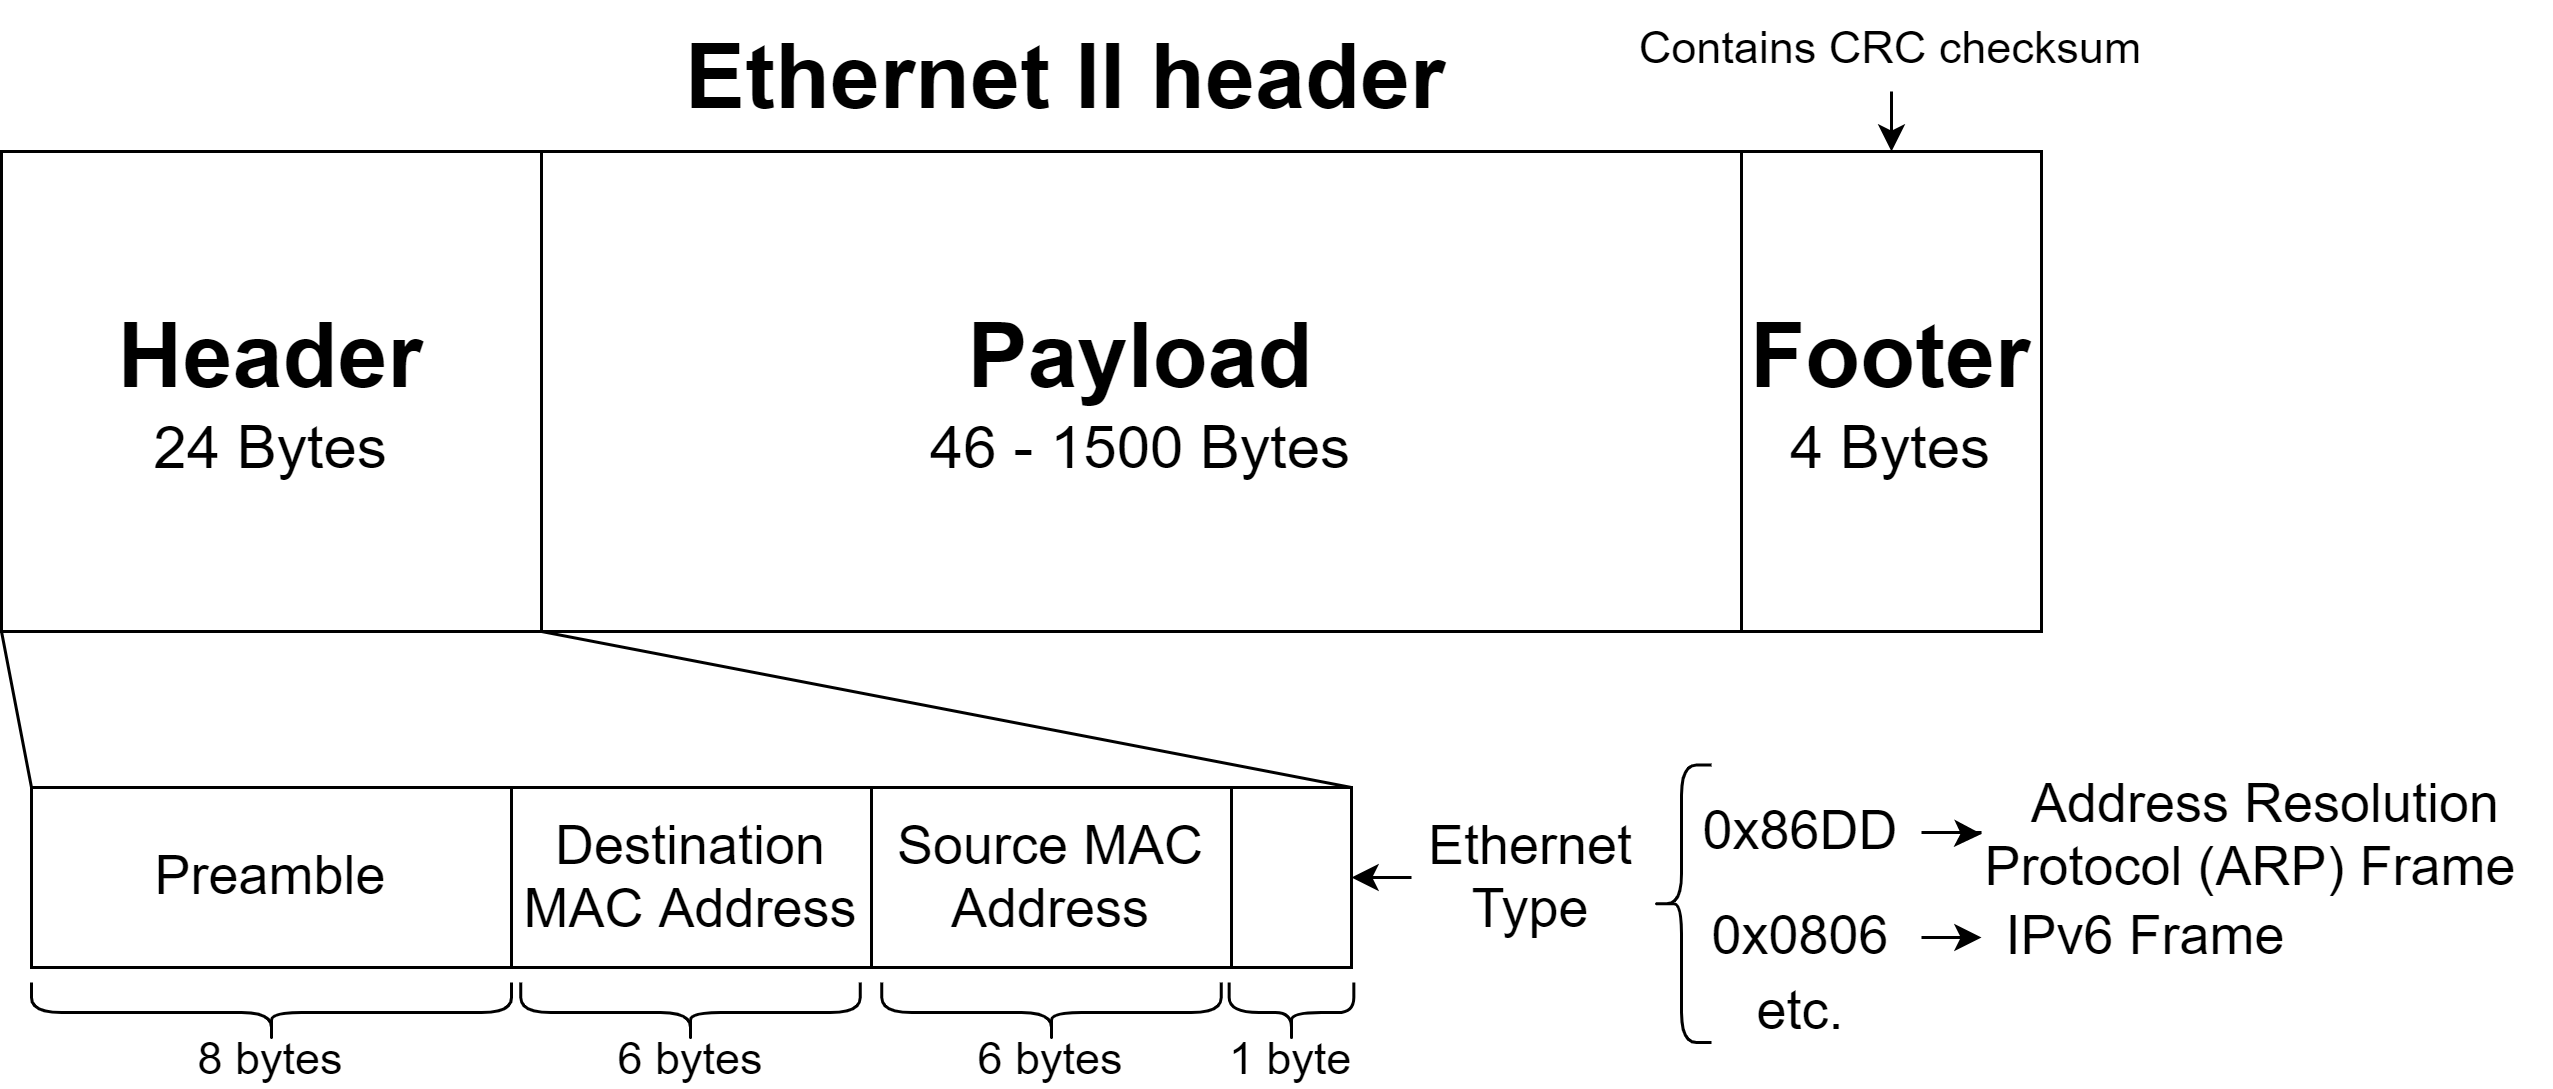
\includegraphics[width=\textwidth]{data_link_layer/images/ethernet frame}\end{center}


\subsection{IEEE MAC Addressing}
\termdef{MAC Address}{
    A $48$ bit ($6$ byte) address etched into IEEE 802 conforming \keyword{NIC}s as a unique identifier an \keyword{NIC}.
    \[<byte>:<byte>:<byte>:<byte>:<byte>:<byte>\]
    \begin{center}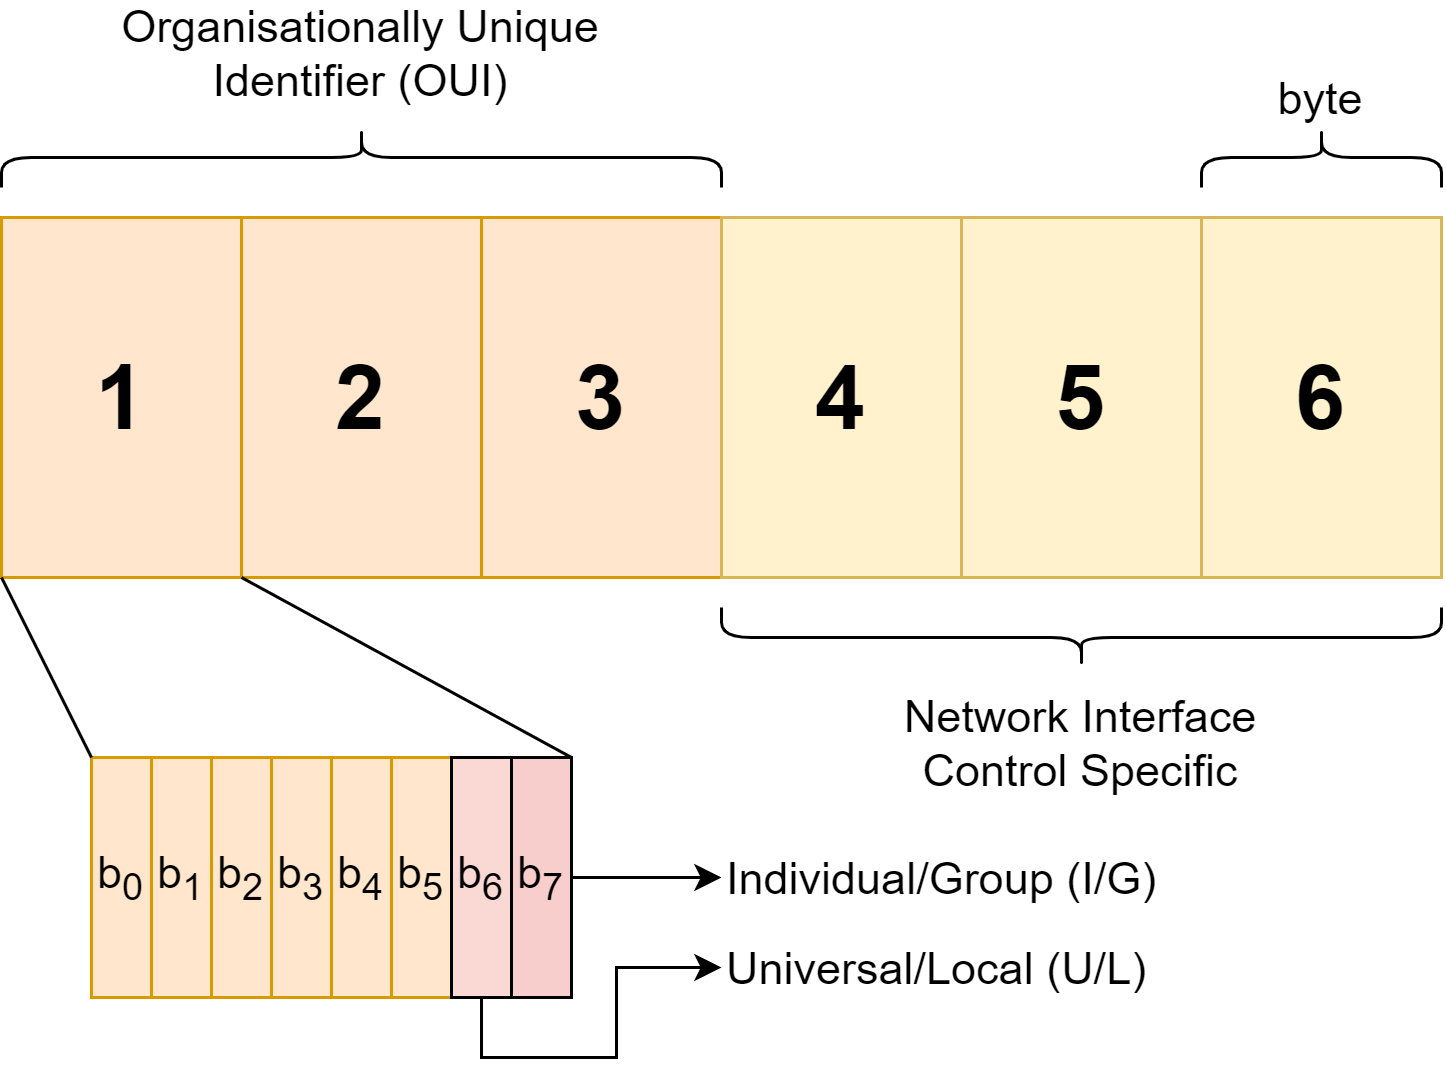
\includegraphics[width=0.7\textwidth]{data_link_layer/images/MAC Address}\end{center}
    \begin{center}
        \begin{tabular}{l c p{0.7\textwidth}}
            \multirow{2}{*}{I/G} & $0$ & Unicast, intended for one \keyword{NIC}.                                                                \\
                                 & $1$ & Multicast, \keyword{NIC} accepts based on other information (e.g list of accepted multicast addresses). \\
            \hline
            \multirow{2}{*}{U/L} & $0$ & Globally Unique, enforced by the \keyword{OUI}.                                                         \\
                                 & $1$ & Locally Unique, e.g new MAC address burned in by network administrator.                                 \\
        \end{tabular}
    \end{center}
    A special address is the \keyword{Broadcast Address} $FF:FF:FF:FF:FF:FF$ (group Multicast, locally administered).
}
It is possible to filter sniffed traffic using mac addresses in applications such as \keyword{WireShark}.
\begin{center}
    \begin{tabular}{l l}
        $eth$                           & All Ethernet based traffic.                            \\
        $eth.addr == 12.00.06.14.3a.fe$ & All traffic to/from MAC Address $12:00:06:14:3a:fe$.   \\
        $eth.addr != <MAC \ Address>$   & All traffic except $<MAC \ Address>$.                  \\
        $!(\dots)$                      & Filter for all except frames traffic matching $\dots$. \\
        $(eth.dst[0] \& 1)$             & Multicast only (bitwise and of 1 and the first byte).  \\
        $!(eth.dst[0] \& 1)$            & Unicast only.                                          \\
        $(eth.dst[0] \& 2)$             & Locally Unique addresses only.                         \\
        $!(eth.dst[0] \& 2)$            & Globally Unique addresses only.                        \\
    \end{tabular}
\end{center}

\subsection{Switch}
\termdef{Switch}{
    \begin{center}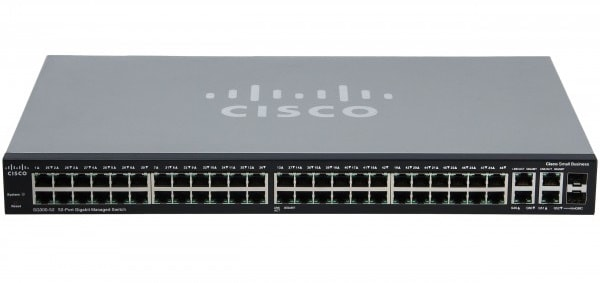
\includegraphics[width=0.7\textwidth]{data_link_layer/images/cisco switch}\end{center}
    Allow many devices to be connected to the same subnet.
    \compitem{
        \item Forwards messages to ports based on the MAC address of the device connected to each port.
        \item If the switch cannot determine which port to send to, it will send to all (flood).
        \item Uses a \keyword{Forwarding Information Base} (\keyword{FIB}) \keyword{MAC} table to remember addresses associated with ports.
        \item Difficult to network-sniff as packets are only directed to intended recipients.
        \item Can connect them to other \keyword{switches} or \keyword{hubs}, allowing networks to be connected together.
        \item Replaced network Bridges.
    }
    To allow messages to leave the subnet, a router and an \keyword{IP Address} provided by a \keyword{DHCP service} or set statically.
}

\subsubsection{Store-and-forward Switching}
Once a whole frame is received, check its integrity using the checksum. If it is correct, forward to the correct port based on the frame's destination \keyword{MAC Address}.
\compitem{
    \item Forwarding is slower, as the switch must wait to recieve the entire frame.
    \item Can check for errors at the switch, and drop the frame if invalid.
    \item Supported by \keyword{bridges} and \keyword{switches}.
}

\subsubsection{Cut-through Switching}
As soon as the enough information is received (e.g the destination address), start forwarding the packet.
\compitem{
    \item Faster forwarding.
    \item Does not error check, so final reciever must check footer checksum.
    \item Only supported by \keyword{switches}.
}


\section{Wireless}
\termdef{Wireless Access Point (WAP)}{
    Standardised by IEEE 802.11 for wireless communication.
    \compitem{
        \item Uses $2.4Ghz$ or $5Ghz$ radio (open for unlicensed use).
        \item Acts as a hub (repeats all recieved)
        \item Can connect \keyword{WPAs} together to extend range.
        \item Can also act as a bridge to connect to a wired network.
    }
    Note that it is very easy to network-sniff, as all devices within range of the \keyword{WPA} can receive frames.
}

\section{Topologies}
\subsection{Switched Ethernet}
\begin{center}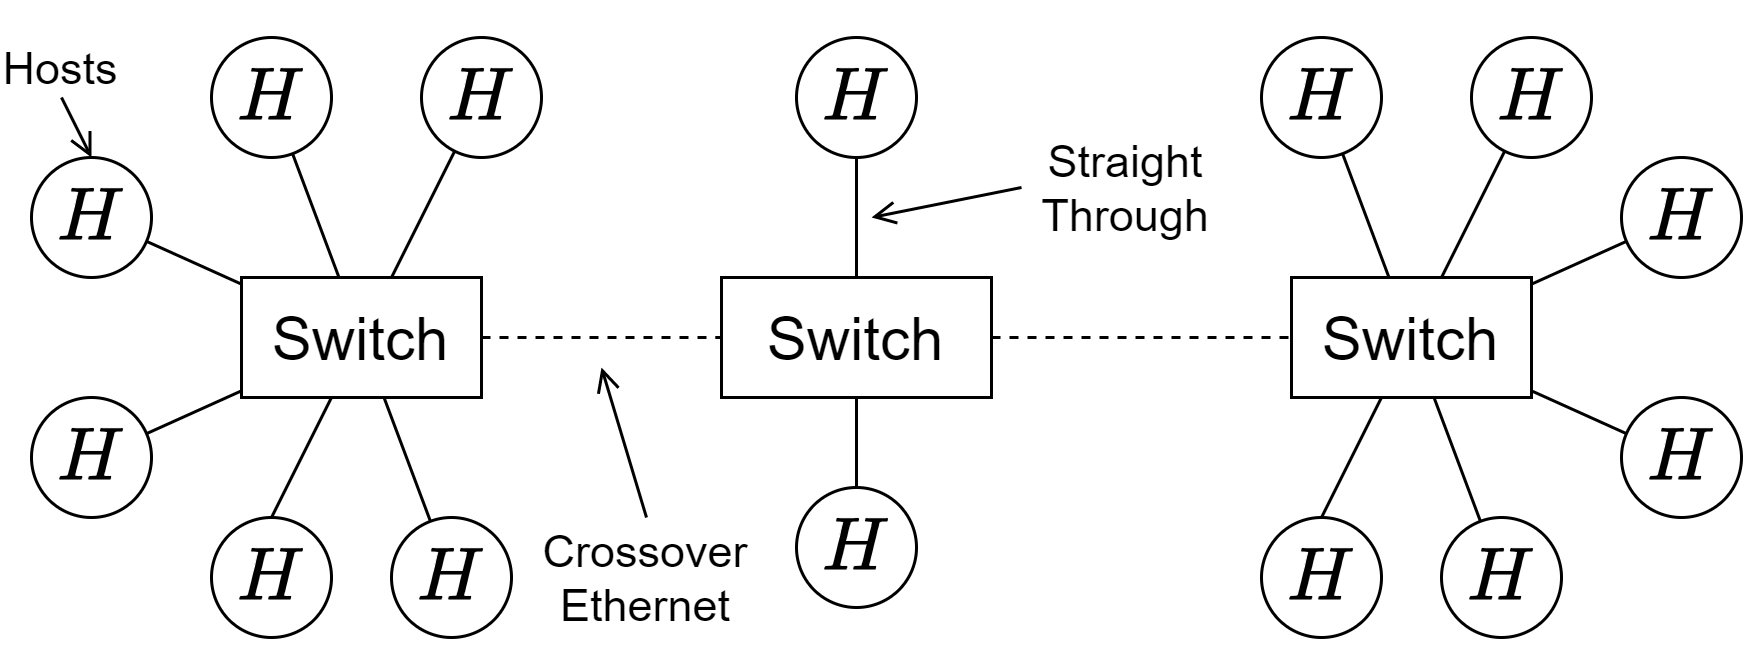
\includegraphics[width=0.9\textwidth]{data_link_layer/images/switched ethernet}\end{center}
\compitem{
    \item Each switch port connected to another machine, or a host.
    \item Collisions avoided using small collision domains (the hosts on a single switch)
    \item Ideal, but expensive.
}


\subsection{Internetworking Ethernet}
\begin{center}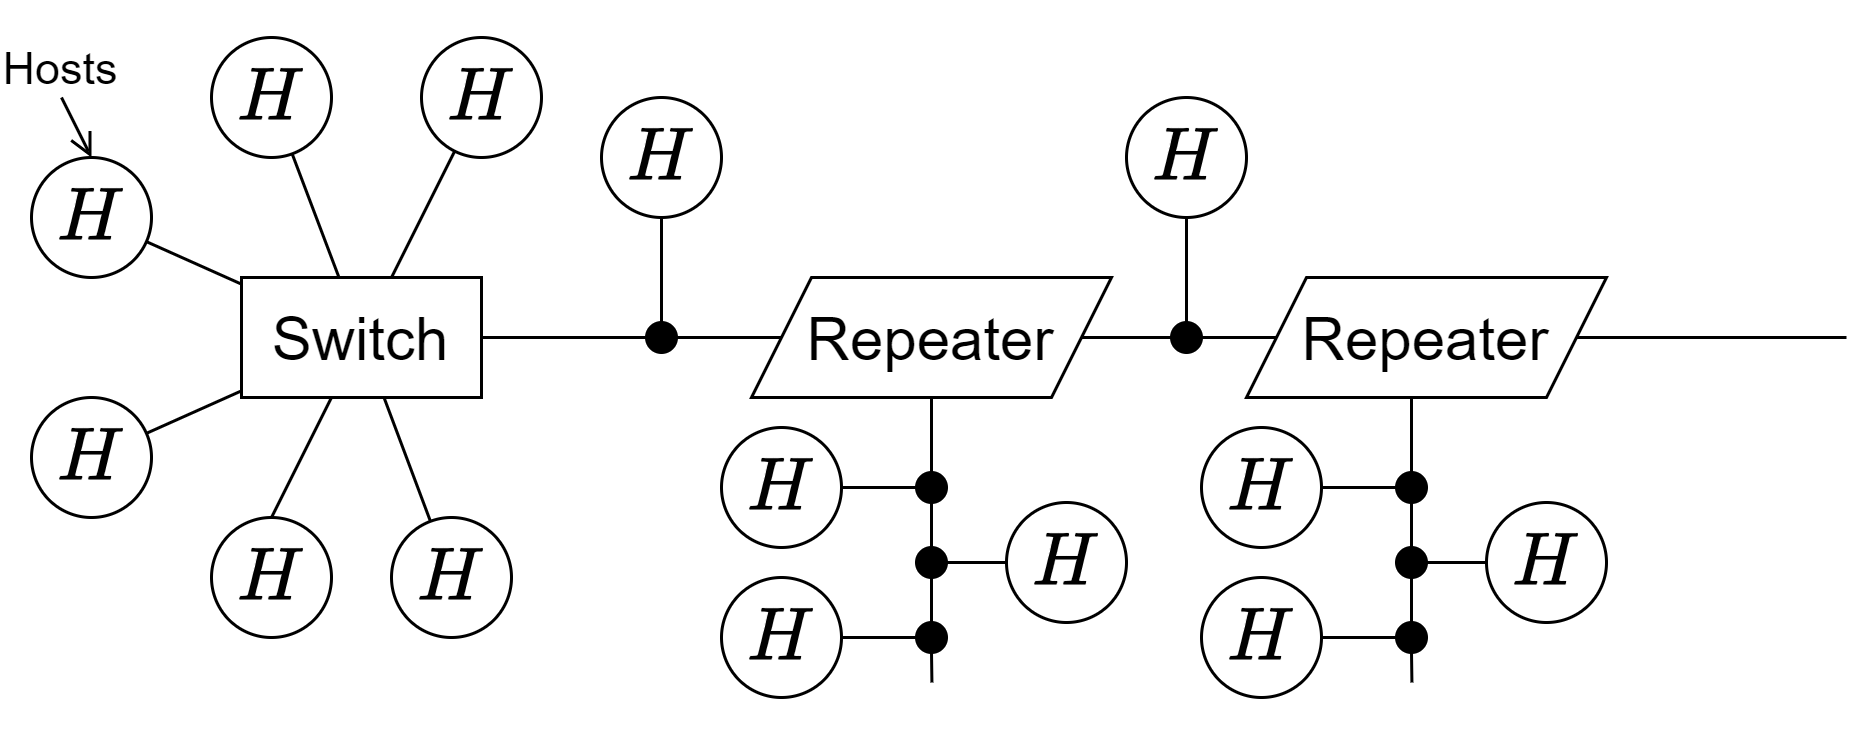
\includegraphics[width=0.9\textwidth]{data_link_layer/images/internetworking ethernet}\end{center}
\compitem{
    \item A combination of networks sharing a medium (e.g a cable).
    \item Repeaters boost signal to extend the range of the network (longer length of cables).
    \item Hubs are used (forward recieved frames out of every port) (use generally discouraged).
}

\subsection{Bus}
\begin{center}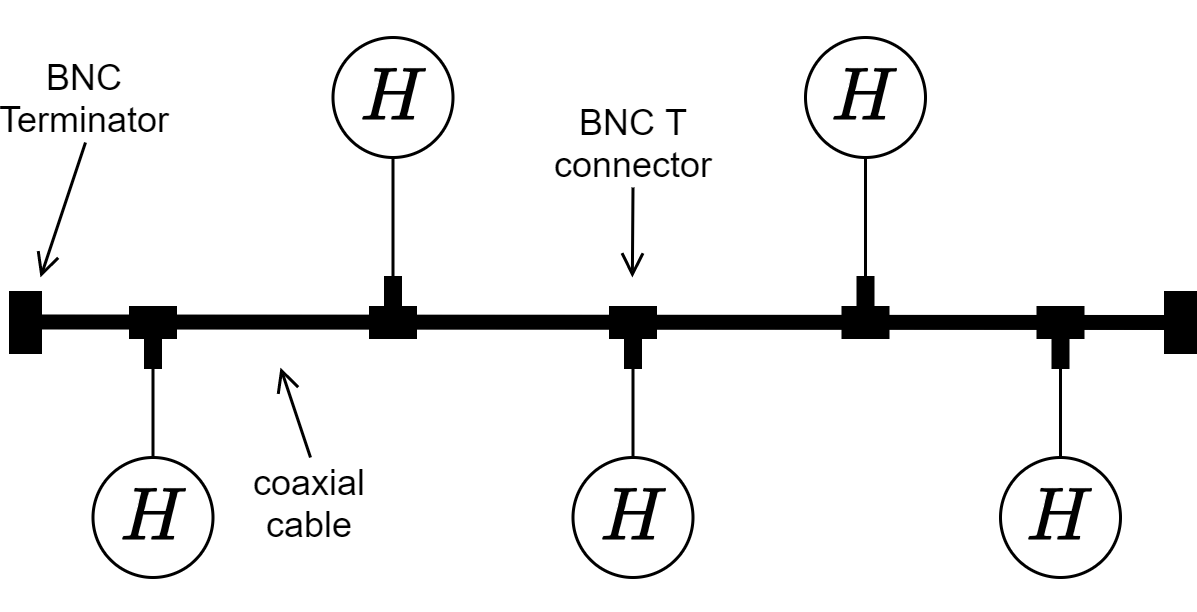
\includegraphics[width=0.9\textwidth]{data_link_layer/images/bus topology}\end{center}
\compitem{
    \item Data travels up and down the \keyword{bus} coaxial cable.
    \item To add new hosts, the cable must be cut, and a \keyword{BNC T} connector used to connect the cable back together with the new host.
    \item Terminators at the end of the cable absorb signals, preventing them from being reflected back down the cable.
}
\sidenote{Cheapernet}{
    10BASE2 is the code for the coaxial cable used for ethernet on \keyword{LAN}s. It is rarely used. The \href{https://en.wikipedia.org/wiki/10BASE2}{wikipedia page} covers the connector types and its replacement.
}

\subsection{Ring}
\begin{center}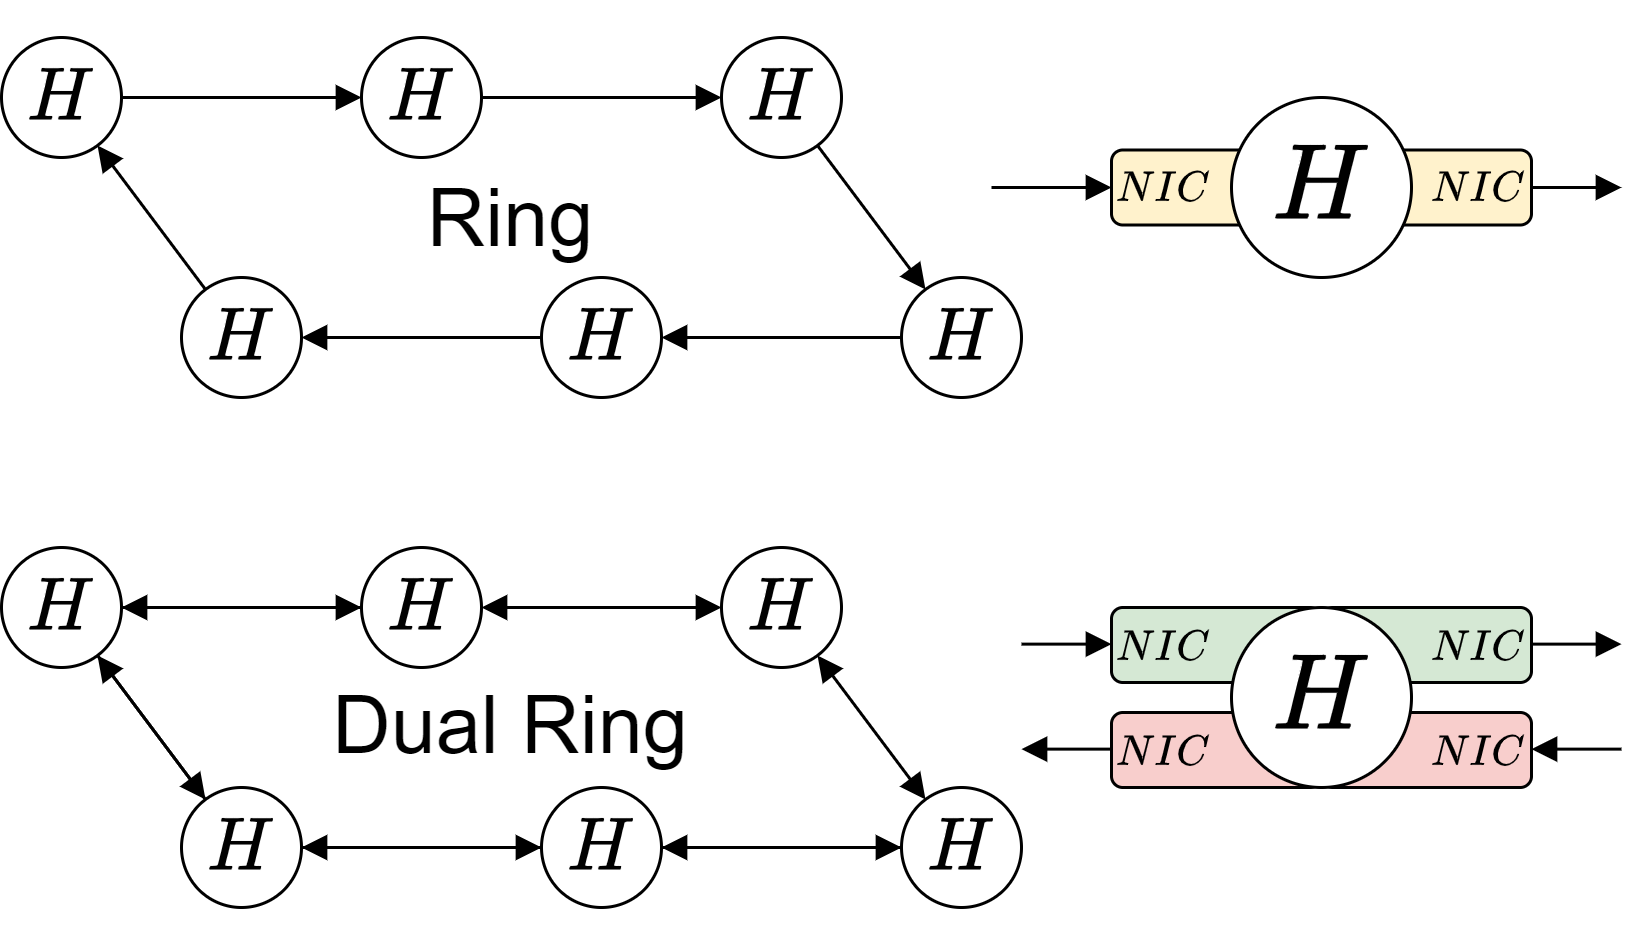
\includegraphics[width=0.9\textwidth]{data_link_layer/images/ring topology}\end{center}
\compitem{
    \item Each host needs two \keyword{NIC}s for \keyword{Ring} and four for \keyword{Dual-Ring}.
    \item If a link is removed, the network fails (every host is a single point of failure) unless the network is designed to adjust (change flow, become a bus).
    \item For \keyword{single-ring} data flows one way, for \keyword{dual-ring} both ways.
    \item \keyword{Dual-Ring} allows for one ring being cut.
}

\subsection{Token Ring (IEEE 802.5)}
\begin{center}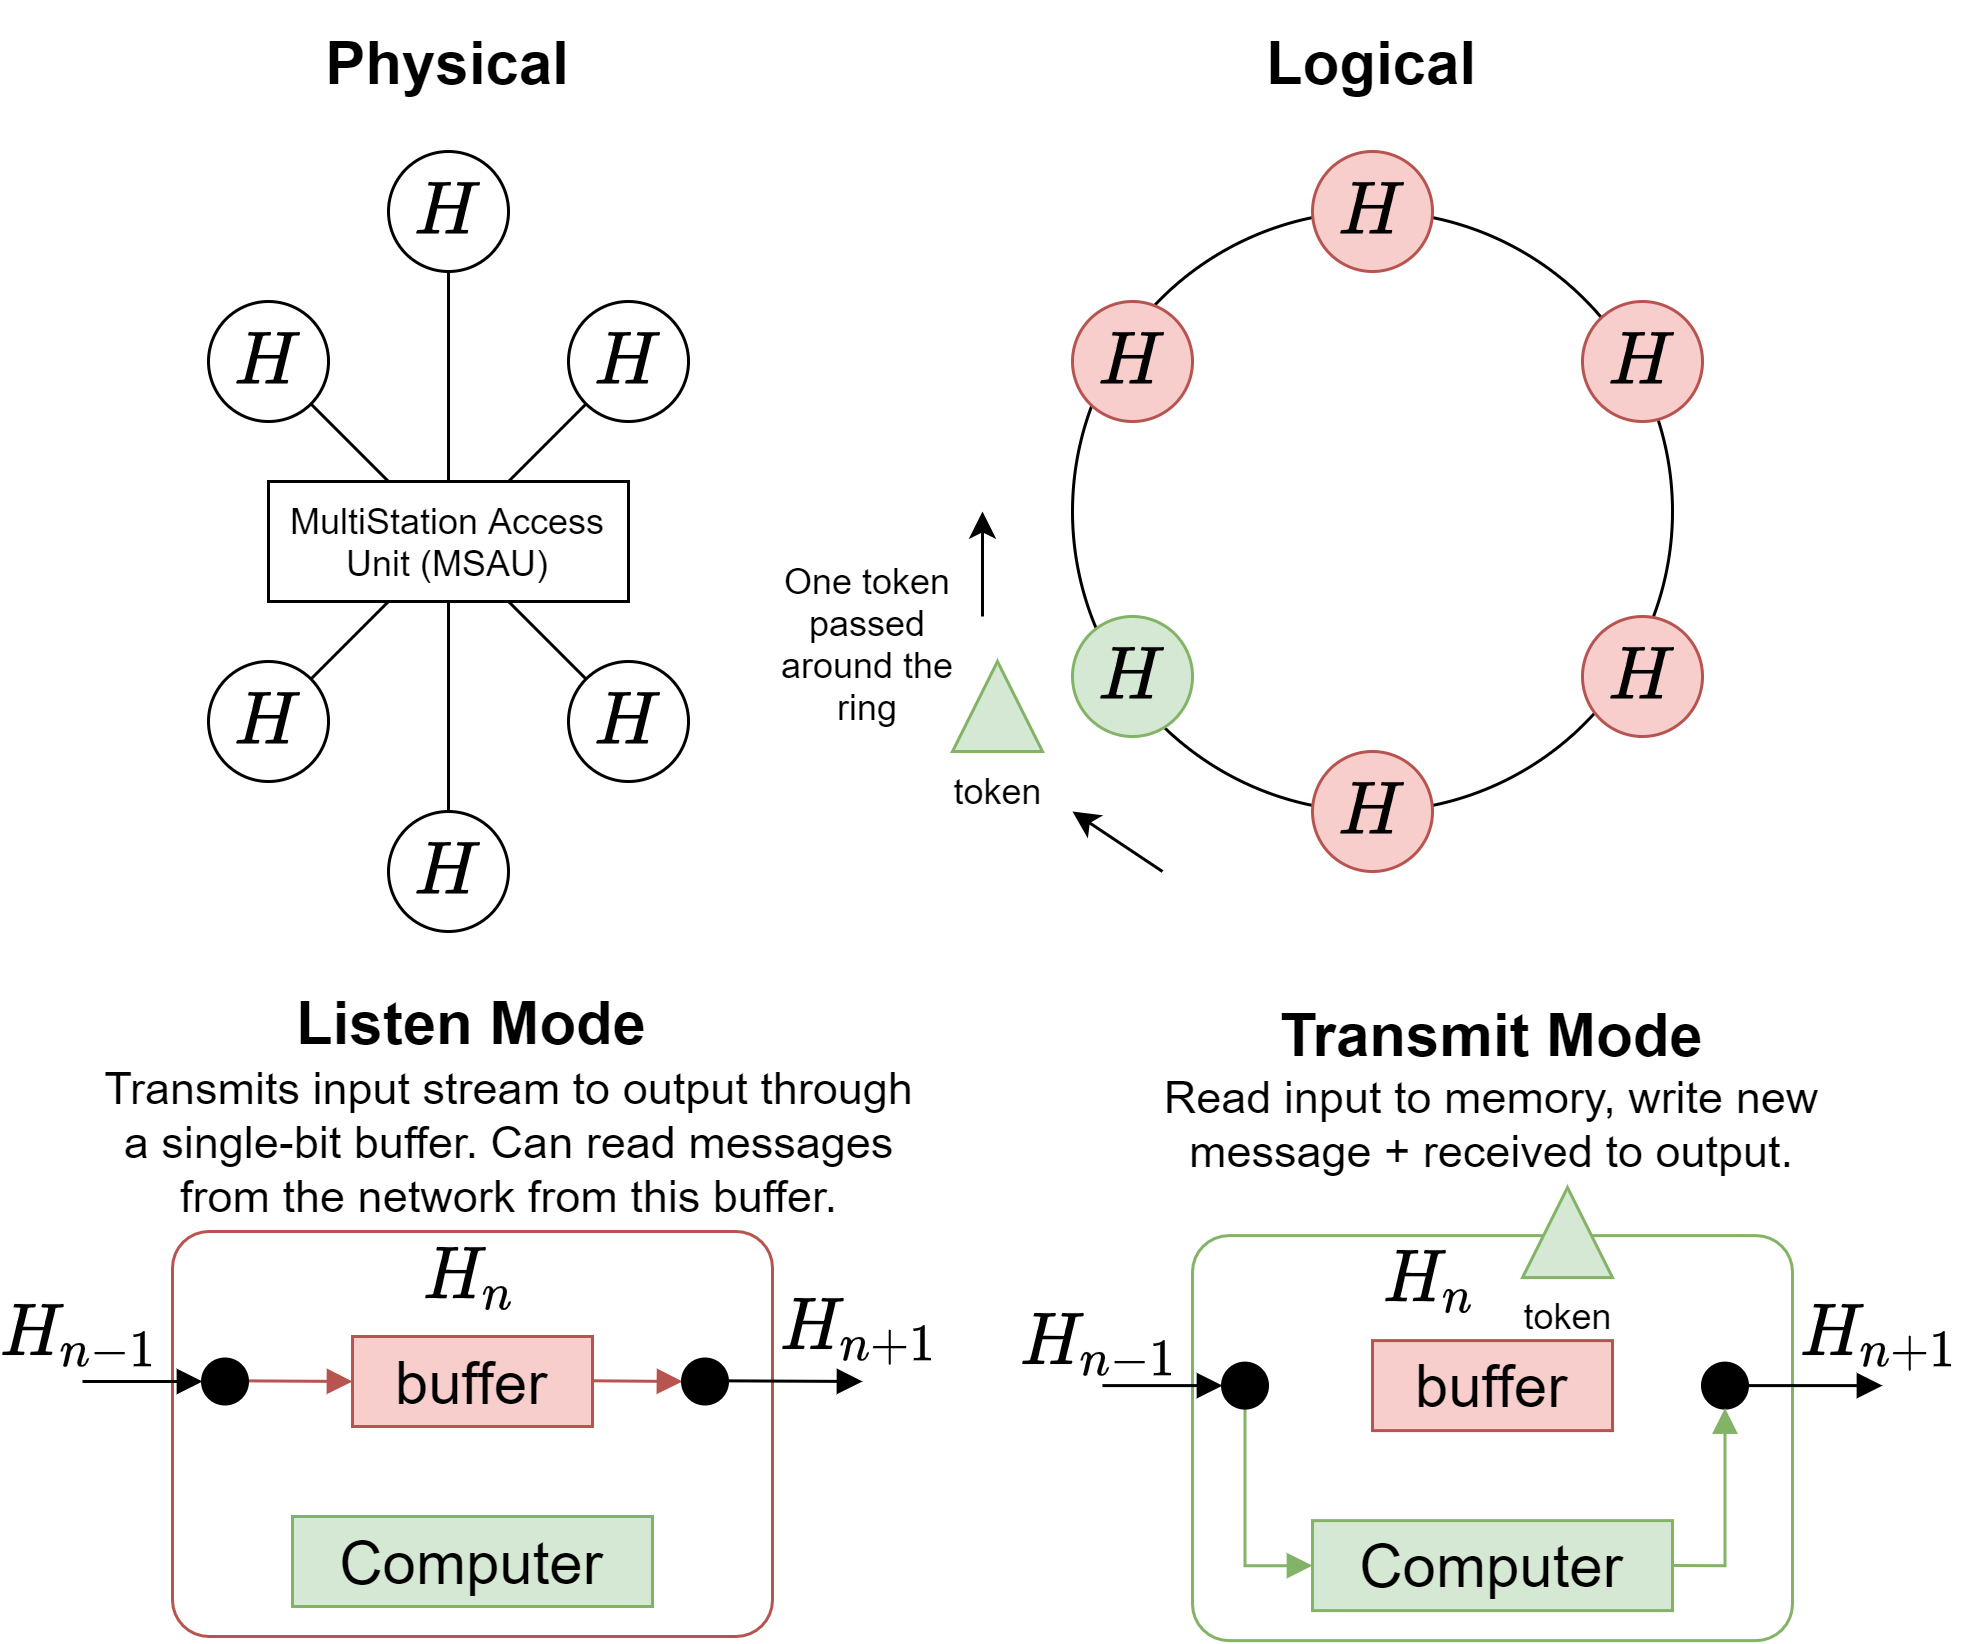
\includegraphics[width=0.9\textwidth]{data_link_layer/images/token ring topology}\end{center}
\compitem{
    \item Hosts connected to the \keyword{Multistation Access Unit} (\keyword{MSAU}), connected logically as a ring.
    \item One host has the token at a time. When a host has the token it is in \keyword{transmit mode} and can write to the network.
    \item No collisions as only one host can have the token \& write at a time.
    \item All hosts can listen to the network (\keyword{listen mode}).
    \item Do not have to worry about frames not fitting inside the ring, as the host holding the token buffers with its own memory.
}
When a host has the token and wants to transmit new data:
\compenum{
    \item Direct all recieved frames to memory.
    \item Write new frame/s to the output.
    \item Wait until the frame written is recieved (meaning it has traversed the entire ring)
    \item Write all recieved (except frame written) to the output.
    \item Pass token to next host.
}
\termdef{Early Release}{
    Hosts do not wait for a sent frame to traverse the ring before passing on the token. This increases the performance considerably.
}
\subsubsection{Token Ring Frames}
\begin{center}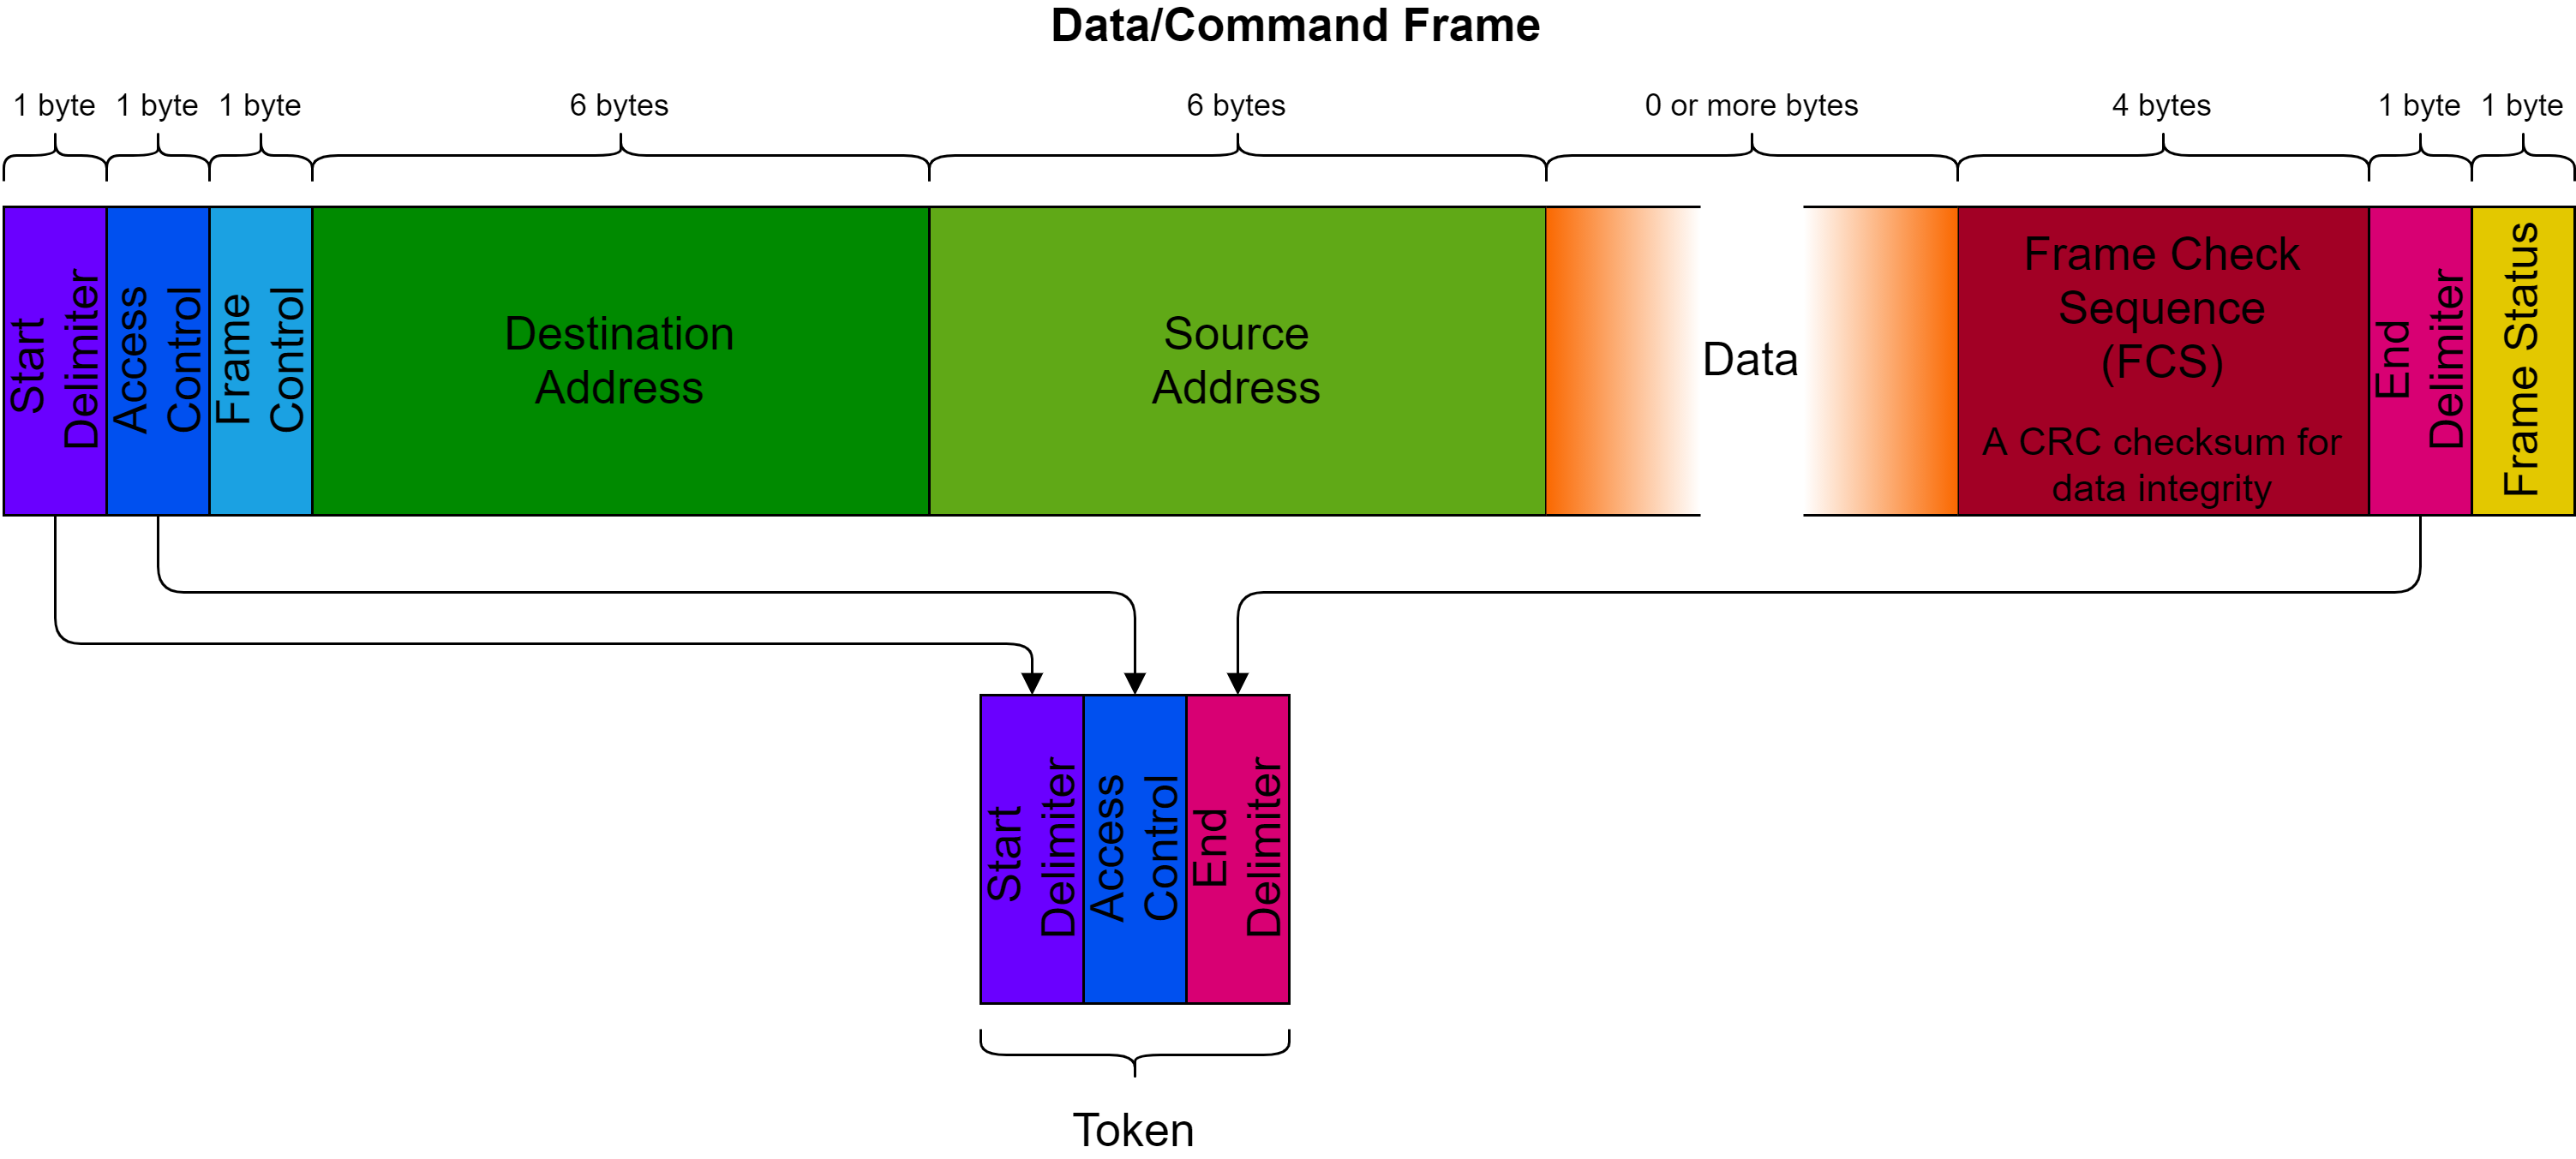
\includegraphics[width=0.9\textwidth]{data_link_layer/images/token ring frame}\end{center}
When there is no frame to be sent, the token is passed around the circle.
\begin{center}
    \begin{tabular}{l l p{0.7\textwidth}}
        \keyword{Frame Check Sequence} & \keyword{FCS} & A \keyword{CRC checksum}  used to ensure data integrity.                                                                                                              \\
        \keyword{Frame Status}         & \keyword{FS}  & Defines if the address was found \& frame received/copied from the ring (set by \keyword{listening mode} destination host). When set it can be removed from the ring. \\
        \keyword{InterFrame Gap}       & \keyword{IFG} & Gaps between frames, smaller gap means less inefficiency, but need enough to recognise the start and end of frames. Defined by the protocol used.                     \\
    \end{tabular}
\end{center}
\subsubsection{Token Ring Priority \& Reservation}
A priority scheme can be implemented so hosts can only claim the token if the priority level of the the data they want to send is as high as the token's priority.
\\
\\A host in \keyword{listen mode} may have high priority data to send. It can raise the reservation priority in the frame. When a token is created,
it is created with the priority of the reservation bits in the frame.
\compitem{
    \item Can claim token if priority of data is as high as token priority.
    \item Low priority data may be delayed indefinitely.
    \item High priority data will be sent quickly (good for real-time applications).
    \item Used for \keyword{LAN}s, so it is assumed we can trust hosts to not abuse priority.
}
\subsubsection{Token Ring Acknowledgement}
The receiver can alter the \keyword{Frame Status}:
\begin{center}
    \begin{tabular}{l l}
        $A = 1$ & Destination host is working.                   \\
        $C = 1$ & Destination host has correctly read the frame. \\
    \end{tabular}
\end{center}
\subsubsection{Ring Maintenance Complexity}
\compitem{
    \item The \keyword{Frame Control} filed is used to create control frames.
    \item Frames may become orphaned (e.g never received, end up looping around indefinitely).
    \item One host is the \keyword{Active Monitor} and is responsible for generating tokens and removing orphaned frames.
    \item \keyword{Active Monitor} may fail, so any host must be able to become the \keyword{Active Monitor}.
    \item Contention rules/protocol needed to determine which host becomes \keyword{Active Monitor}.
}
The above points add significant complexity to token passing and reduce reliability.
\termdef{Wiring Concentrators}{
    In order to improve reliability, when a host fails it can be bypassed.
    \begin{center}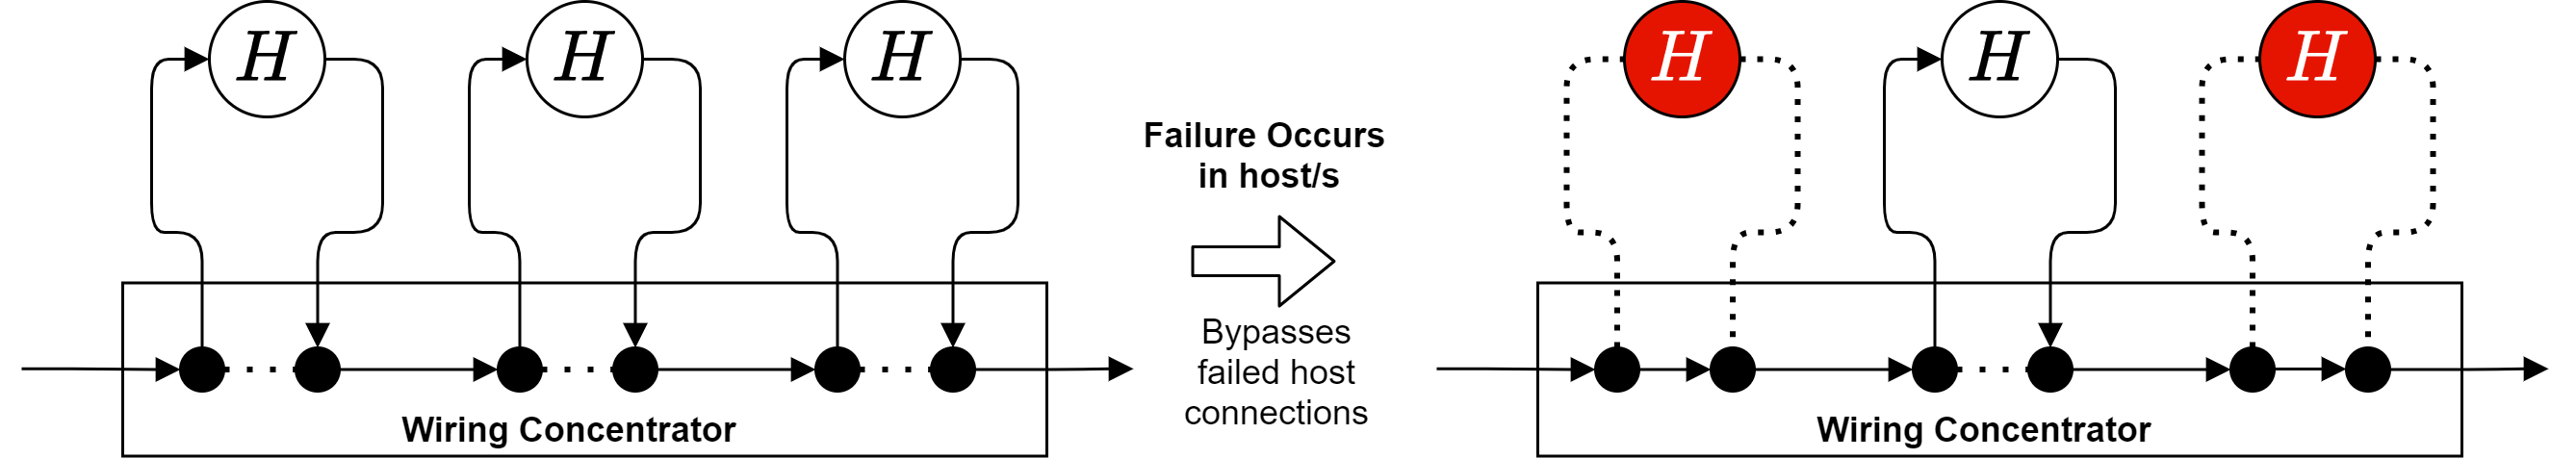
\includegraphics[width=0.9\textwidth]{data_link_layer/images/wiring concentrator}\end{center}
}

\subsection{Fibre Distributed Data Interface (FDDI)}
\begin{center}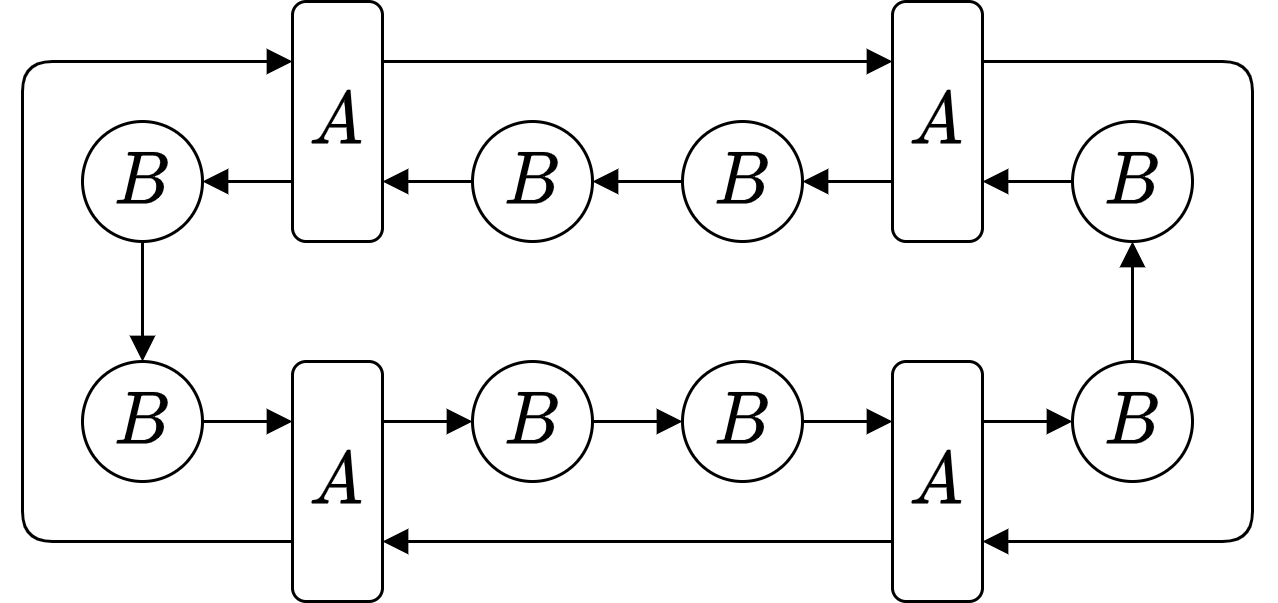
\includegraphics[width=0.8\textwidth]{data_link_layer/images/fibre distributed data interface}\end{center}
A ring-based token passing topology that was popular in the 1990s.
\\
\\ Hosts are divided into two classes, with one class (in our diagram class $A$) connected to both rings.
\compitem{
    \item Optical fibre cabling allows for networks to be geographically large.
    \item When a class $B$ fails, data can be re-routed through class $A$ hosts and the second ring.
    \item When a class $A$ fails we can short-circuit two class $A$s to create a single-ring (connecting two rings at disconnected ends).
    \item Rings can be up to $100km$ long, so FDDI must work with a length up to $200km$.
    \item No longer a popular.
}


\subsection{Star}
\begin{center}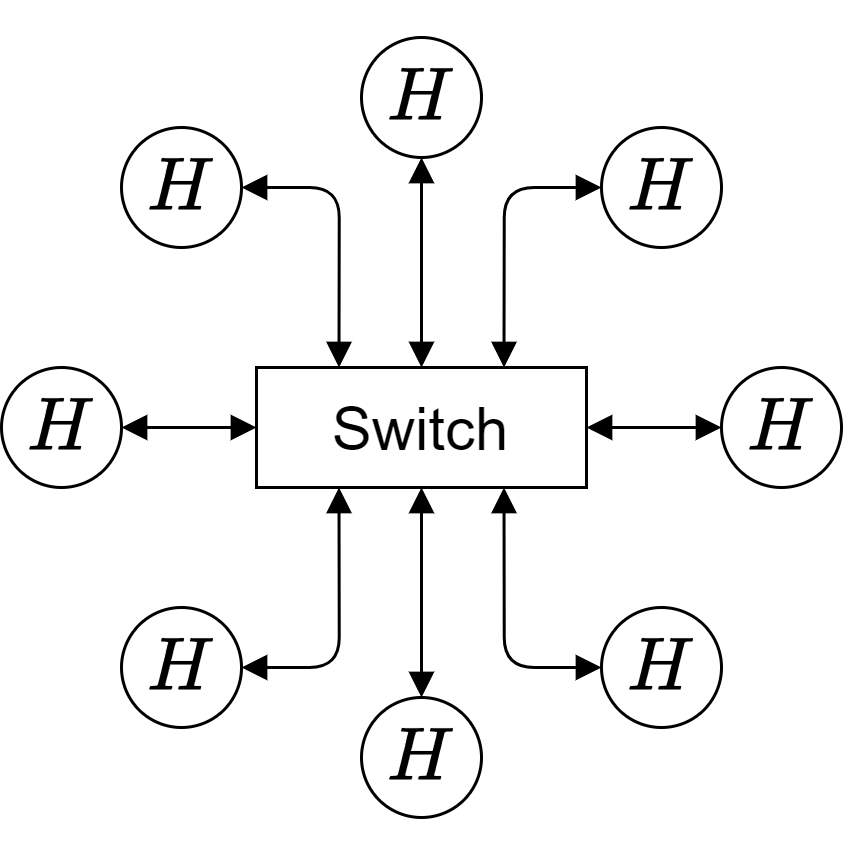
\includegraphics[width=0.5\textwidth]{data_link_layer/images/star topology}\end{center}
\compitem{
    \item All hosts connected directly to a \keyword{switch/multiport-bridge}.
    \item Any host can communicate with any other (provided they have a mechanism to prevent them talking over eachother).
    \item The central \keyword{switch} is a single point of failure (entire network fails it it fails).
}

\subsection{Other Topologies}
\begin{center}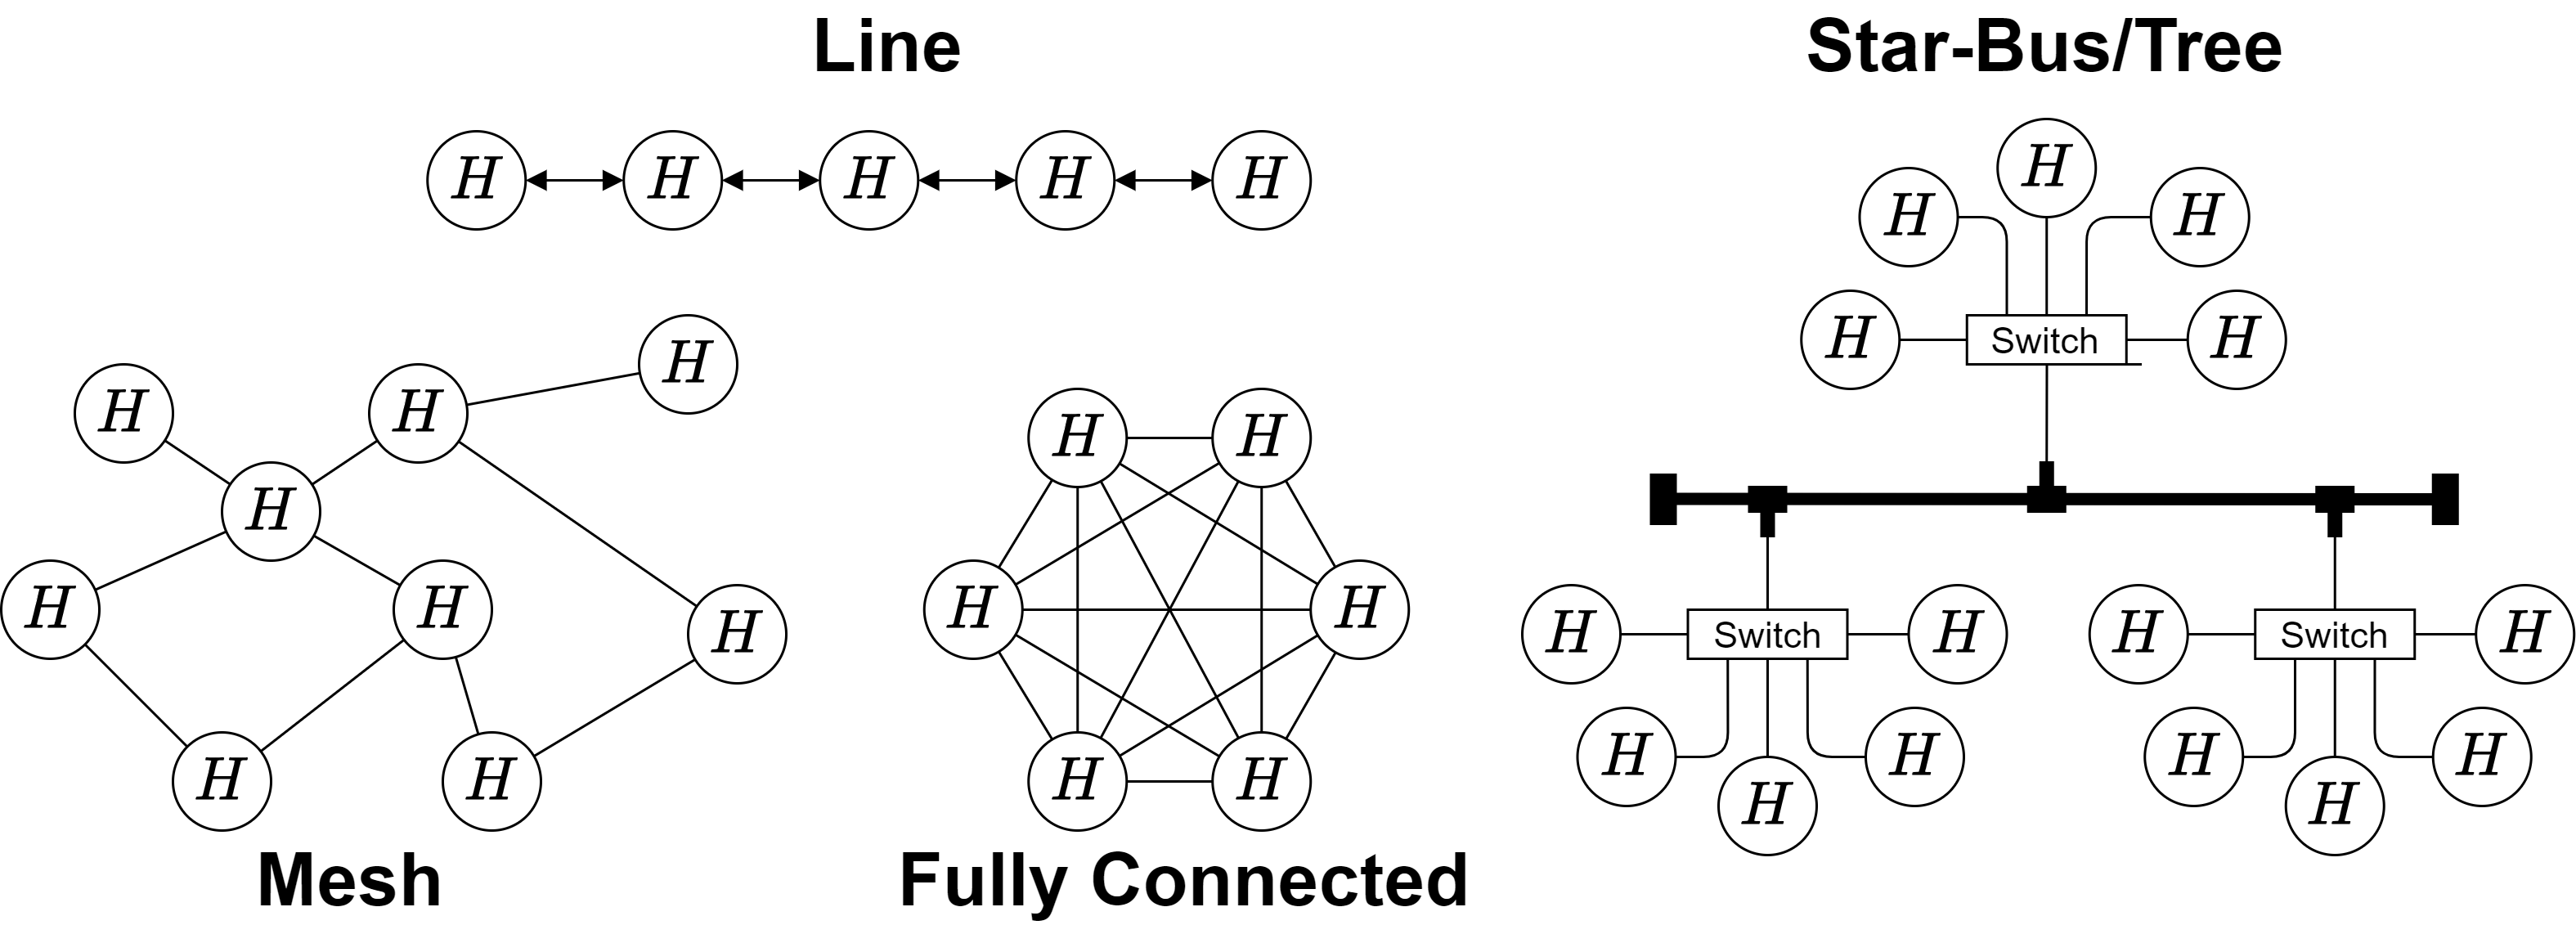
\includegraphics[width=0.9\textwidth]{data_link_layer/images/other topologies}\end{center}
\compitem{
    \item Line is terrible (Split Ring).
    \item Star-Bus/Tree is a hybrid.
    \item Mesh is useful in some scenarios, but can be expensive.
    \item Mesh is ultra-fast (every host connected directly to every other host), but very expensive \& difficult/nearly-impossible to effectively manage.
}

\section{MAC}
\begin{center}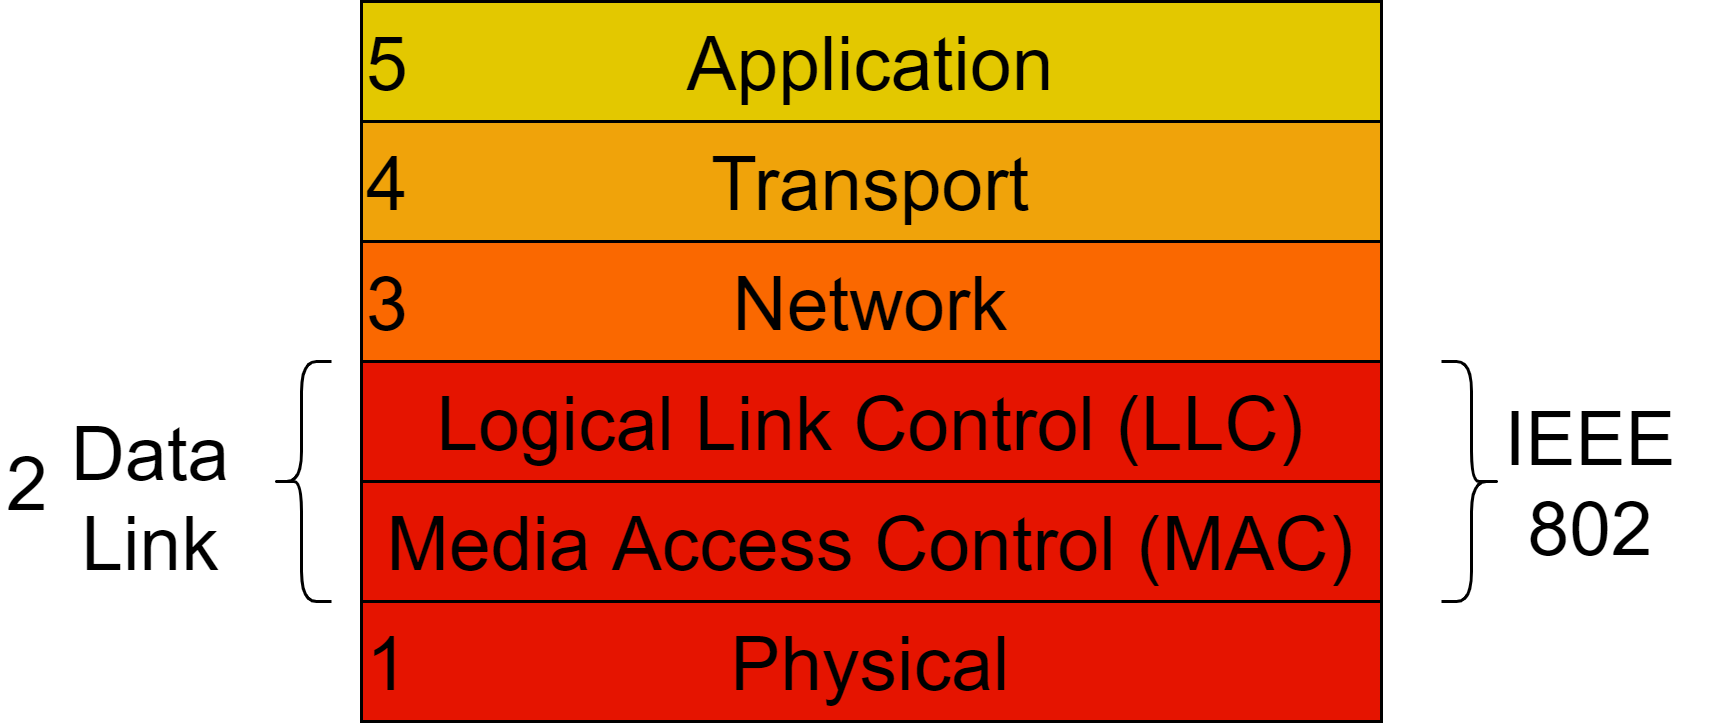
\includegraphics[width=0.5\textwidth]{data_link_layer/images/data link layer division}\end{center}
In \keyword{token ring} only one host can transmit at a time. However with other network types this is not the case.
\\
\\ For example a \keyword{broadcast} channel can have multiple receiving hosts \& multiple concurrent transmissions can result in \keyword{frame} collisions.
\\
\\ We use \keyword{Medium Access Control} to coordinate channel access.
\sidenote{Stations}{
    In these notes the term \keyword{station} is used to describe a host transmitting on the shared medium.
}
\compitem{
    \item In a wired network, frame collisions result in both frames needing to be re-transmitted.
    \item In a wireless network one transmitter may be stronger/a frame may be recieved even with a collision.
}

\subsection{Medium Access Control Strategies}
\subsubsection{No Control}
\compitem{
    \item When a frame is not recieved, the station retransmits as it pleases.
    \item Fine if channel ultilisation is low.
    \item Inefficient when contention is high (lots of transmitting stations $\to$ constant collisions \& attempted re-transmissions).
}
\subsubsection{Round Robin}
\compitem{
    \item Stations take turns to transmit.
    \item Used in \keyword{token-based} \keyword{MAC} systems (only the station with the token can transmit).
}
\subsubsection{Reservations}
\compitem{
    \item Stations obtain \textit{channel reservations} prior to transmitting.
    \item Stations can only transmit for the time interval they have reserved.
    \item Requires a system to manage reservations.
    \item Used in \keyword{slotted} systems.
}
\subsection{Static Channel Allocations}
Where each station is allocated a fixed schedule of times it is allowed to transmit.
\\
\\ For a channel shared between $n$ different stations:
\begin{itemize}
    \bullpara{Time Division Multiplexing (TDM)}{
        \\ Stations waits for its time slot to transmit. each station's transmission rate limited to $\cfrac{R}{n}$ where $R = $ maximum channel rate.
    }
    \bullpara{Frequency Division Multiplexing}{
        \\ Stations given a limited frequency band. Each station can use $\cfrac{B}{n}$ where $B = $ total channel bandwidth.
        \\
        \\ Bad for large $n$ or traffic that is in bursts.
    }
\end{itemize}

\subsection{Dynamic Channel Allocation}
\termdef{ALOHA Protocol}{
    Stations transmit whenever they want to. If a collision occurs, stations wait a random period of time before attempting to re-transmit.
    \begin{center}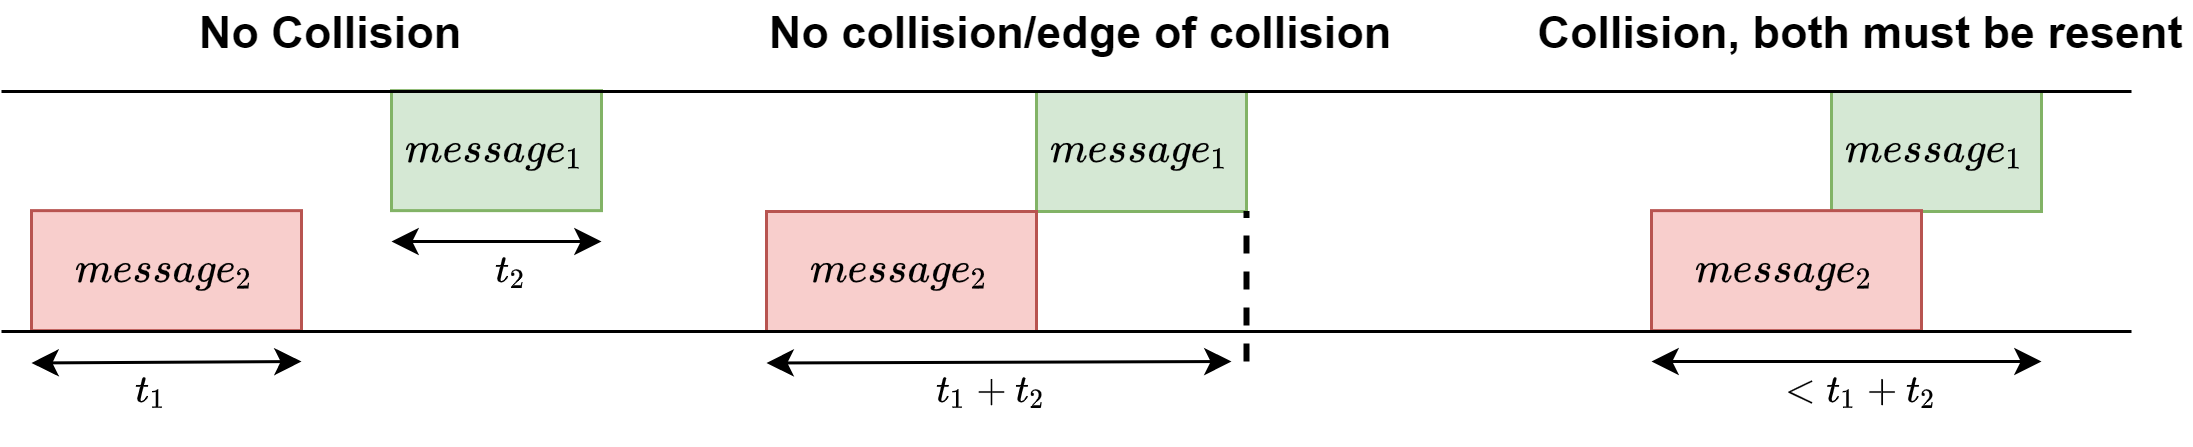
\includegraphics[width=\textwidth]{data_link_layer/images/aloha vulnerability}\end{center}
    \compitem{
        \item The protocol suffers from low channel efficiency (worse with more contention) as there is a large \keyword{vulnerable period}.
        \item If a frame transmission is interrupted by another at any point, the both frames must be re-transmitted (new frames can destroy old frames).
        \item Maximum efficiency of $18\%$ at $50\%$ load.
    }
}
\termdef{Slotted ALOHA Protocol}{
    Like \keyword{ALOHA} but can only transmit on specific discrete time intervals (slots) (managed by a synchronous global clock).
    \begin{center}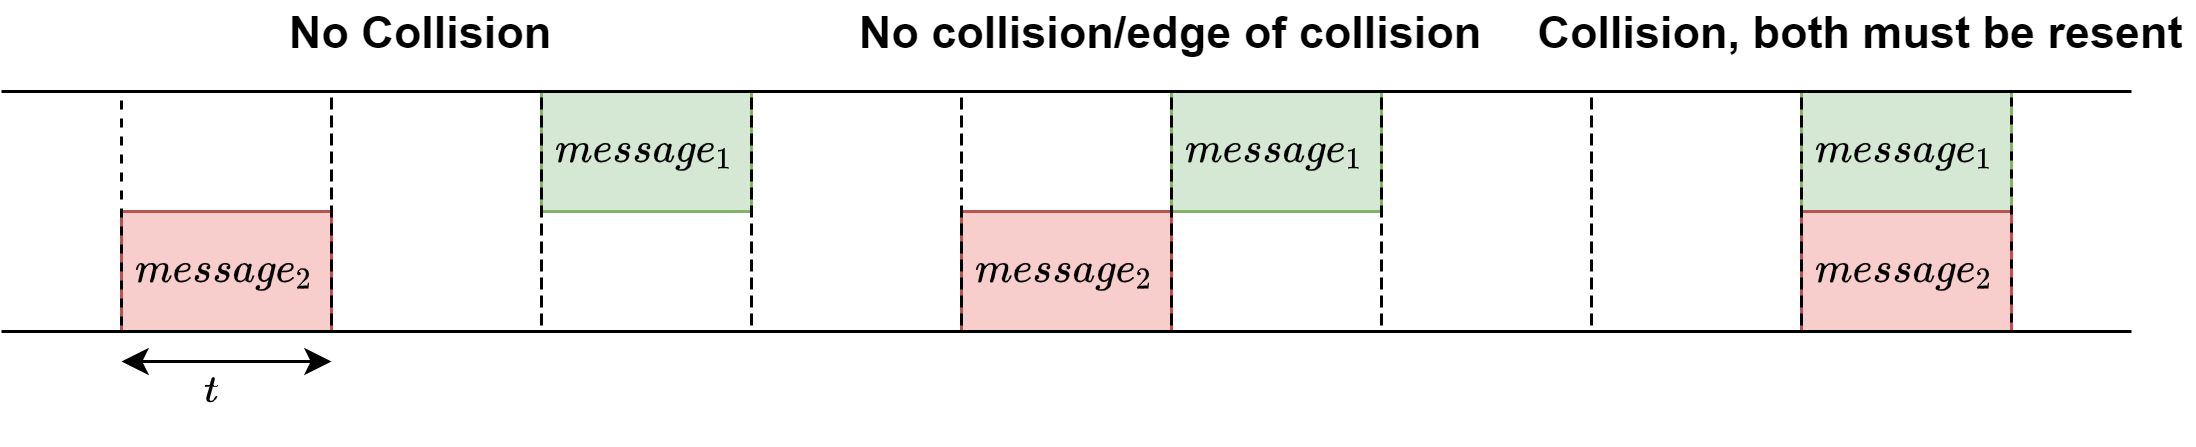
\includegraphics[width=\textwidth]{data_link_layer/images/slotted aloha}\end{center}
    \compitem{
        \item Reduces opportunities for a new frame to collide with an old one.
        \item Can only collide with exact overlap (contention for a slot)
        \item Maximum efficiency of $36\%$ at $100\%$ load.
    }
}

\example{ALOHA Comparison}{
    Given hosts start transmitting at times $H_1: 80, H_2: 33, H_3: 72, H_4: 35, H_5: 51$ plot their transmissions and determine which transmissions collide given frames sent are $20s$ long.
    \begin{center}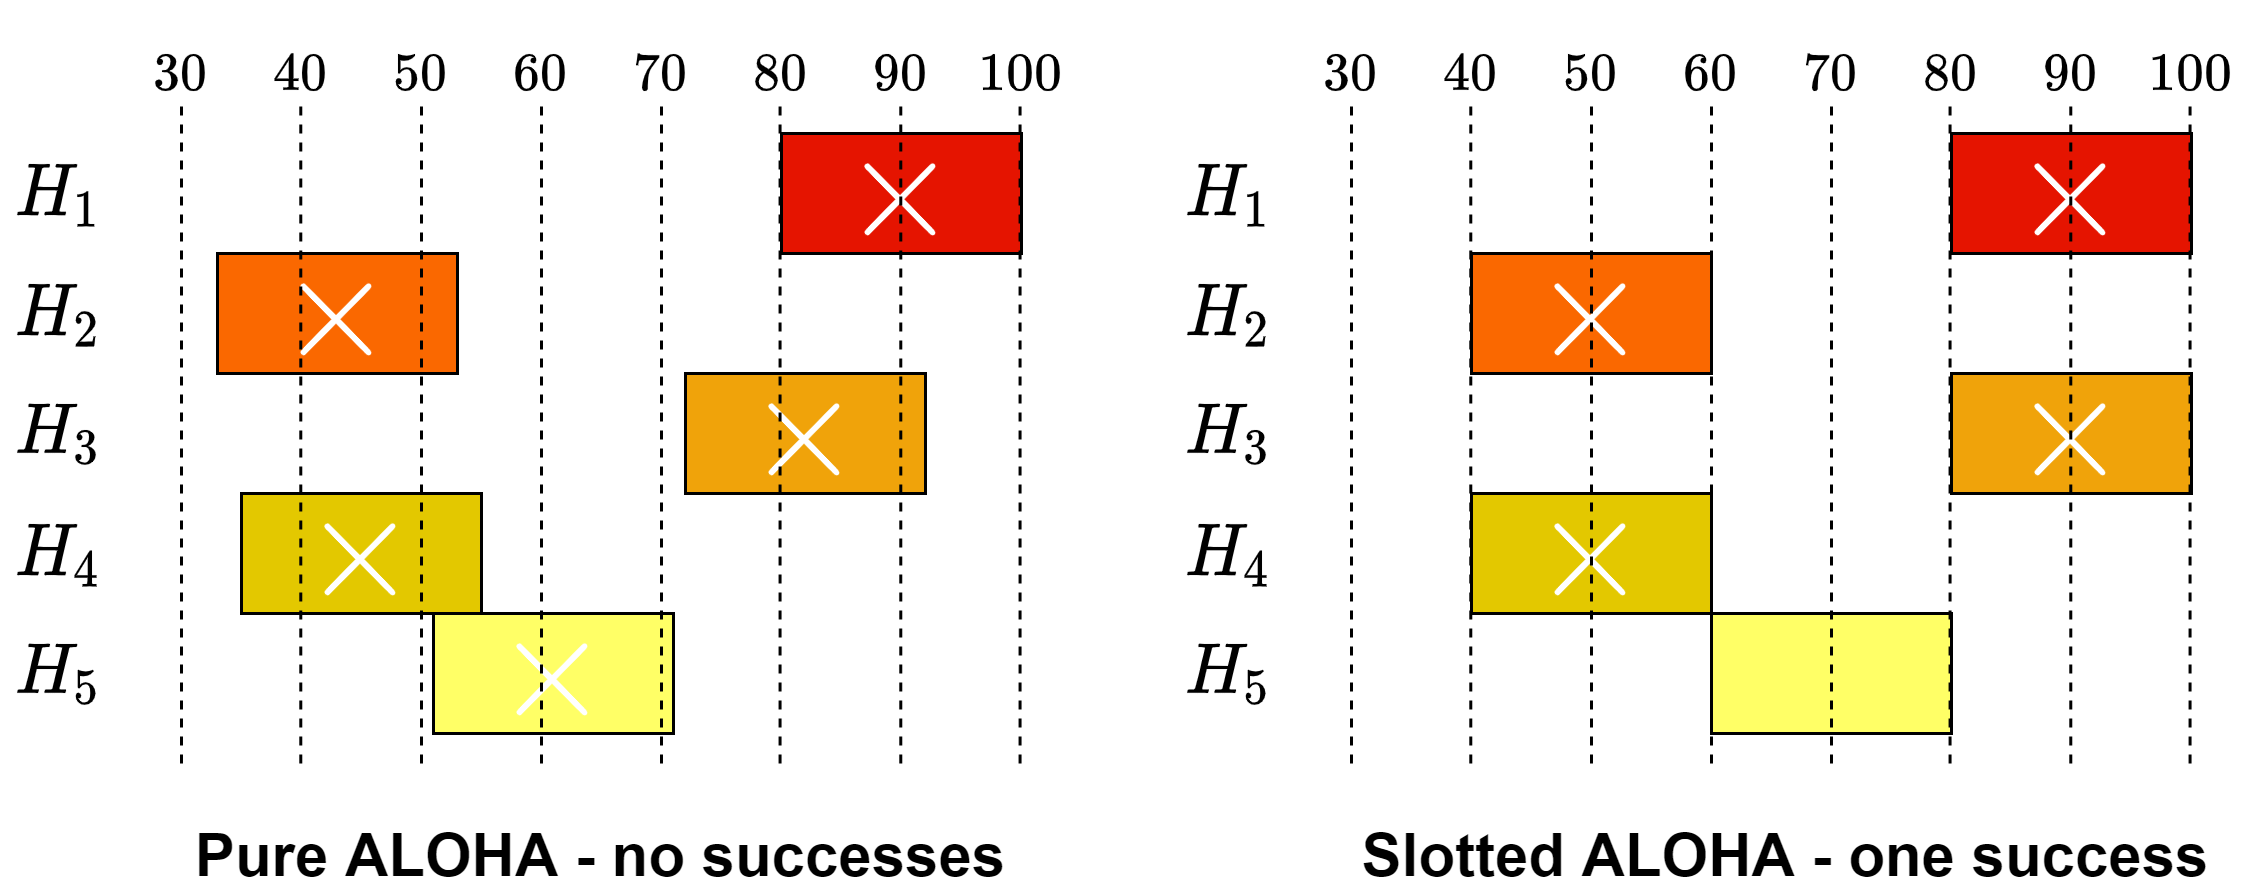
\includegraphics[width=0.9\textwidth]{data_link_layer/images/aloha example}\end{center}
}
\subsection{Carrier Sense Multiple Access (CSMA)}
\termdef{Carrier Sensing}{
    Listen before transmitting, transmission only occurs when the channel is idle/free.
    \compitem{
        \item Reduces collisions over \keyword{ALOHA} as new frames are not sent during another's transmission.
        \item Collisions can still occur due to transmission delay (e.g two stations see idle channel, start transmitting, or one starts transmitting after another, but signal has yet to reach it).
    }
}
\begin{tabular}{l l l l}
    CSMA/CD & Collision Detection & Ethernet & IEEE 802.3  \\
    CSMA/CA & Collision Avoidance & WiFi     & IEEE 802.11 \\
\end{tabular}

\subsection{Carrier Sense Multiple Access / Collision Detection (CSMA/CD)}
Used for \keyword{ethernet} (wired networking), all collisions result in frames being destroyed.
\compitem{
    \item Station listens to channel during transmission to check for collisions.
    \item Transmission stop when collision detected, then sends a \keyword{jamming signal} (other transmitter will see the \keyword{jamming signal} and hence also know a collision has occurred).
    \item Host must transmit long enough to be able to tell the frame has not been collided. Hence minimum frame length is $2\eta$ where $\eta =$ end-to-end transmission delay.
}
\sidenote{Required Delay}{
    \begin{center}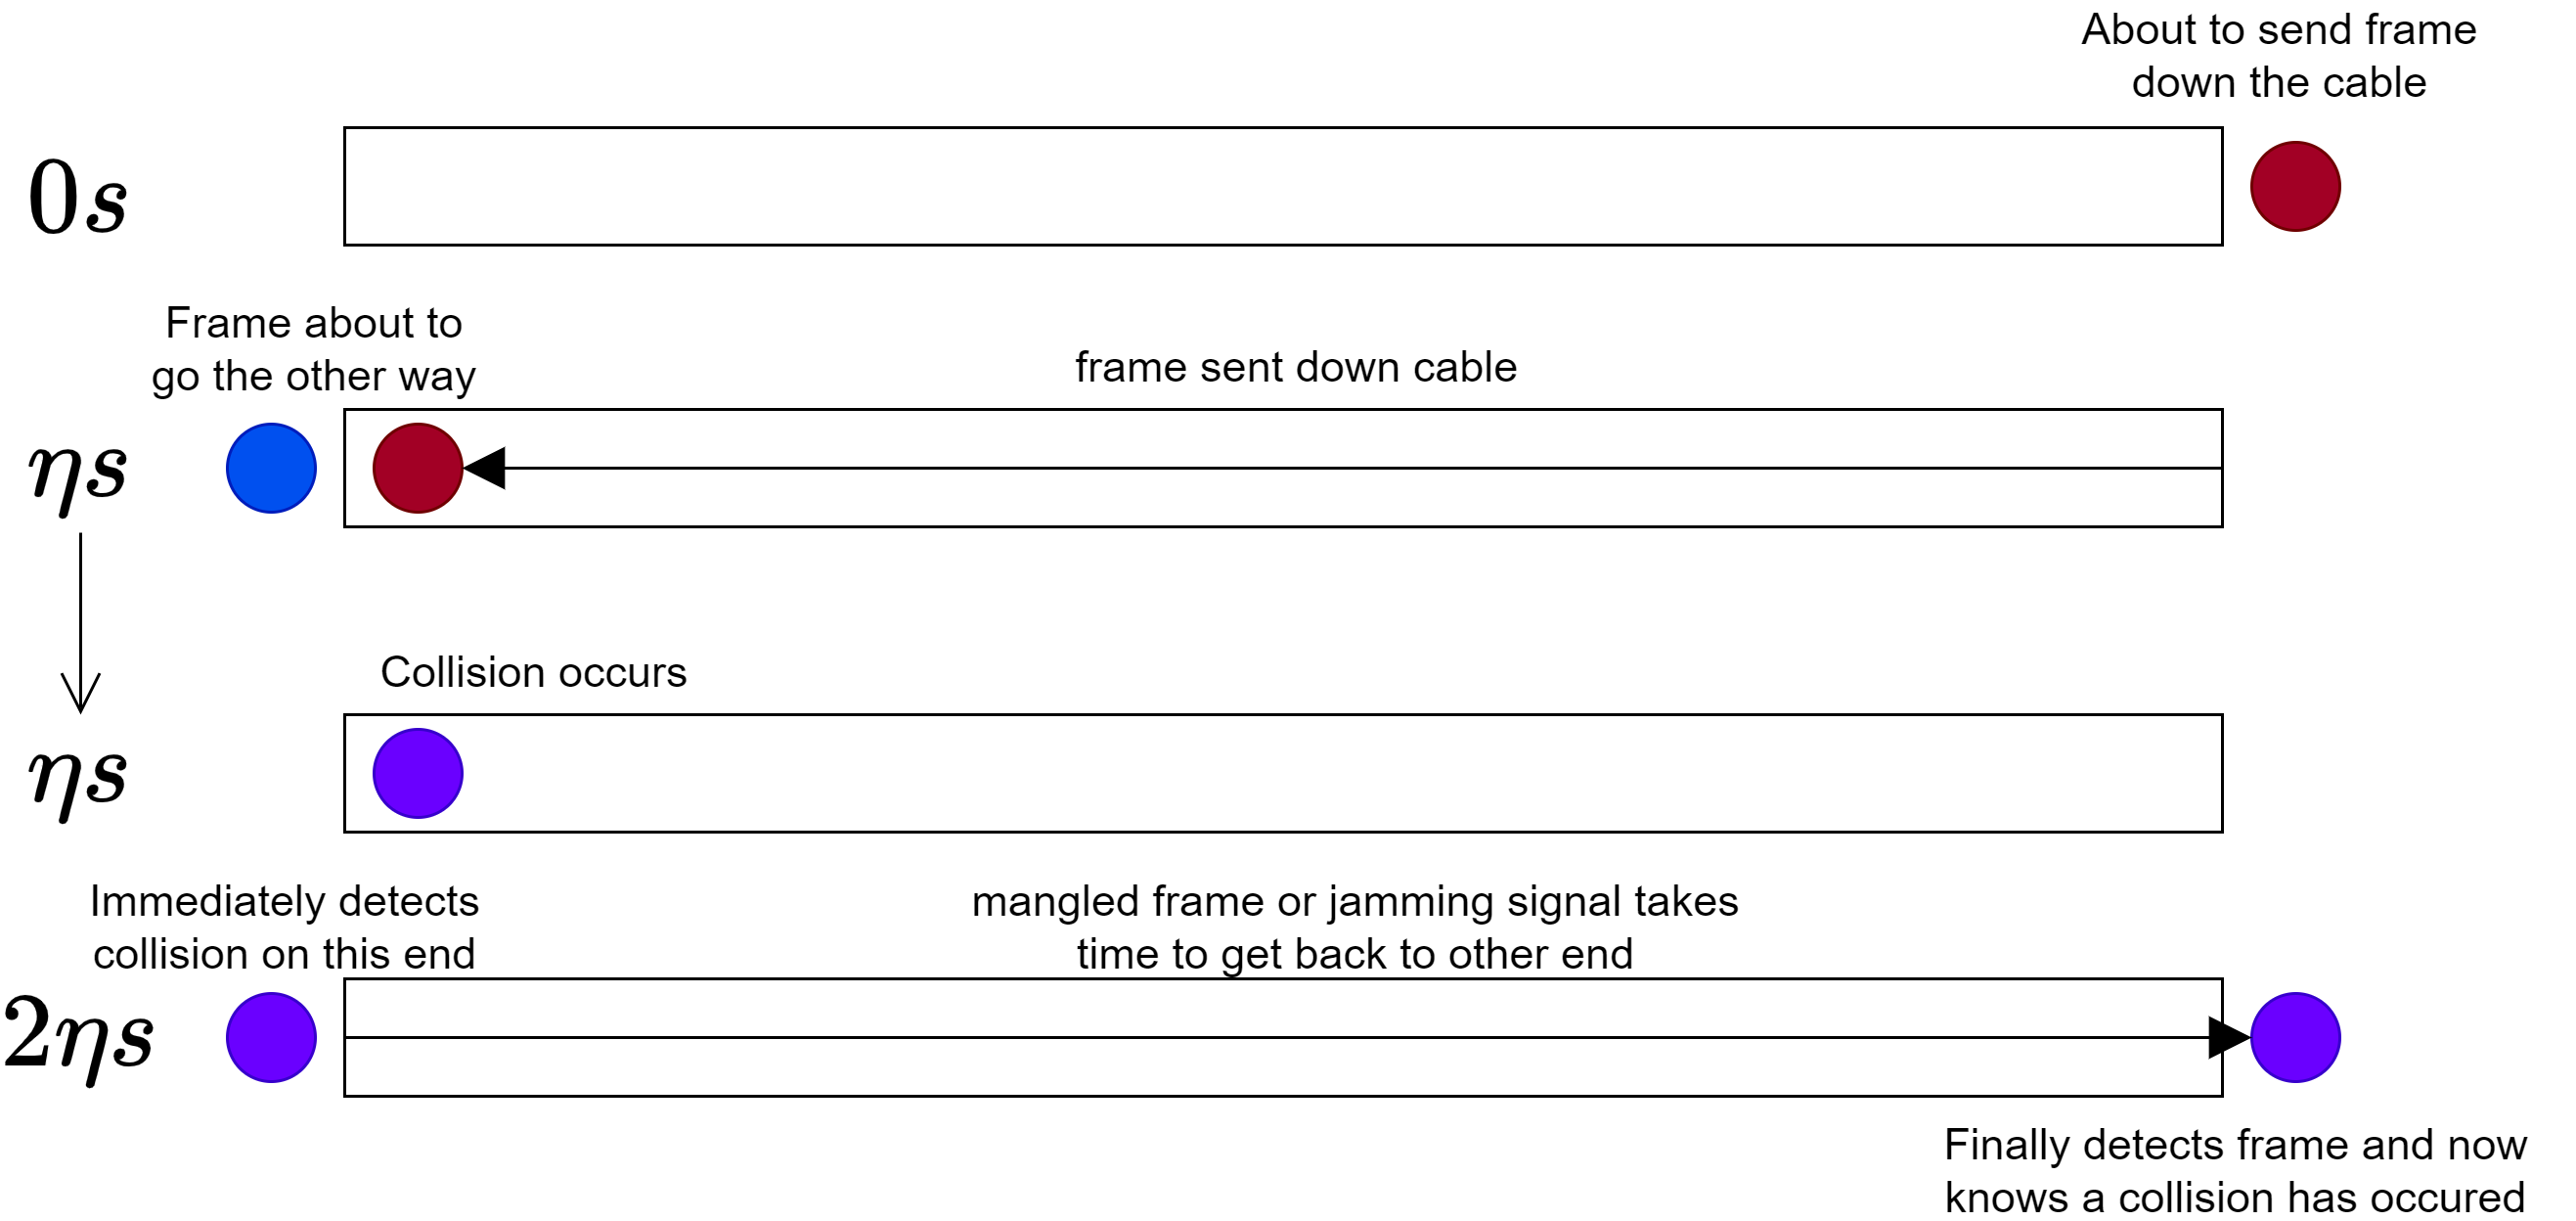
\includegraphics[width=0.9\textwidth]{data_link_layer/images/ethernet carrier collision example}\end{center}
    The minium size is required as we may not know the first bit (in the above example) has collided until $2\eta s$ after sending.
    \\
    \\ If the first bit does not collide (reaches end) then we have the line until we stop sending (as other side will not send while channel is not idle/free).
    \\
    \\ If the first bit does collide, then we should stop sending and attempt to recover (e.g resend using some policy/protocol).
    \\
    \\ If the frame is not large enough, we will stop transmitting (and hence holding the channel) before we know if a collision may have occurred.
}
Collisions are inevitable as there is no central authority controlling transmission. Hence it is a best-effort service, in the worst case a frame may be indefinitely delayed.
\compitem{
    \item Suitable for most \keyword{LANs}
    \item Unacceptable for real-time systems (these require maximum wait time and minimum bandwidth assurances).
}

\termdef{Carrier Extension}{
    There is a minimum frame size requirement (to hold channel until bits reach destination), so for some frames an extension is required.
    \begin{center}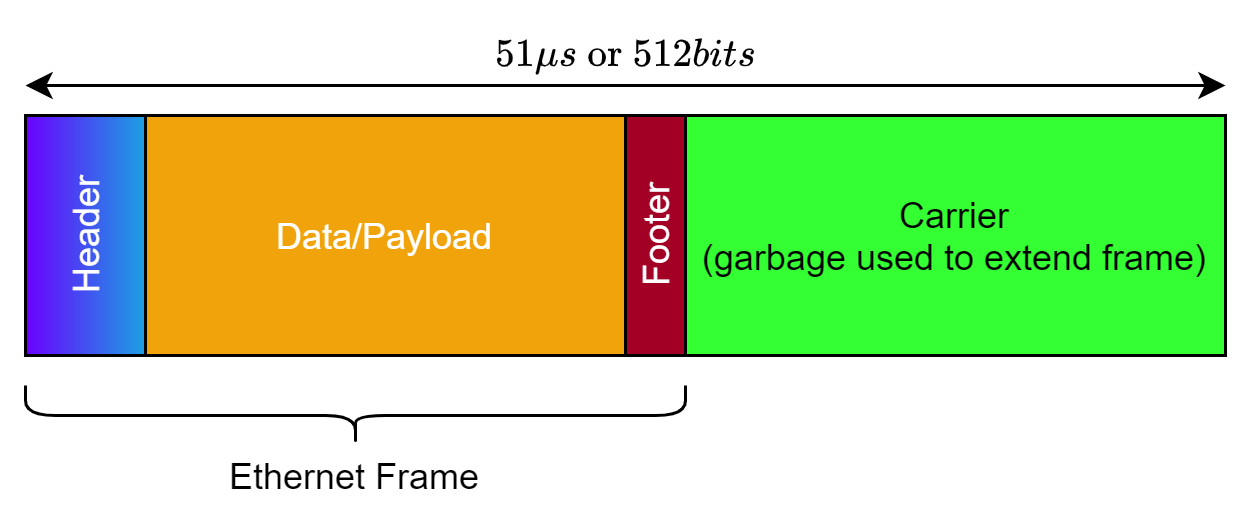
\includegraphics[width=0.7\textwidth]{data_link_layer/images/carrier extension}\end{center}
    The wasted time transmitting the extension makes this inefficient.
}

\termdef{Frame Bursting}{
    Rather than padding with an extension, multiple frames are buffered, then packet together and sent at once.
    \begin{center}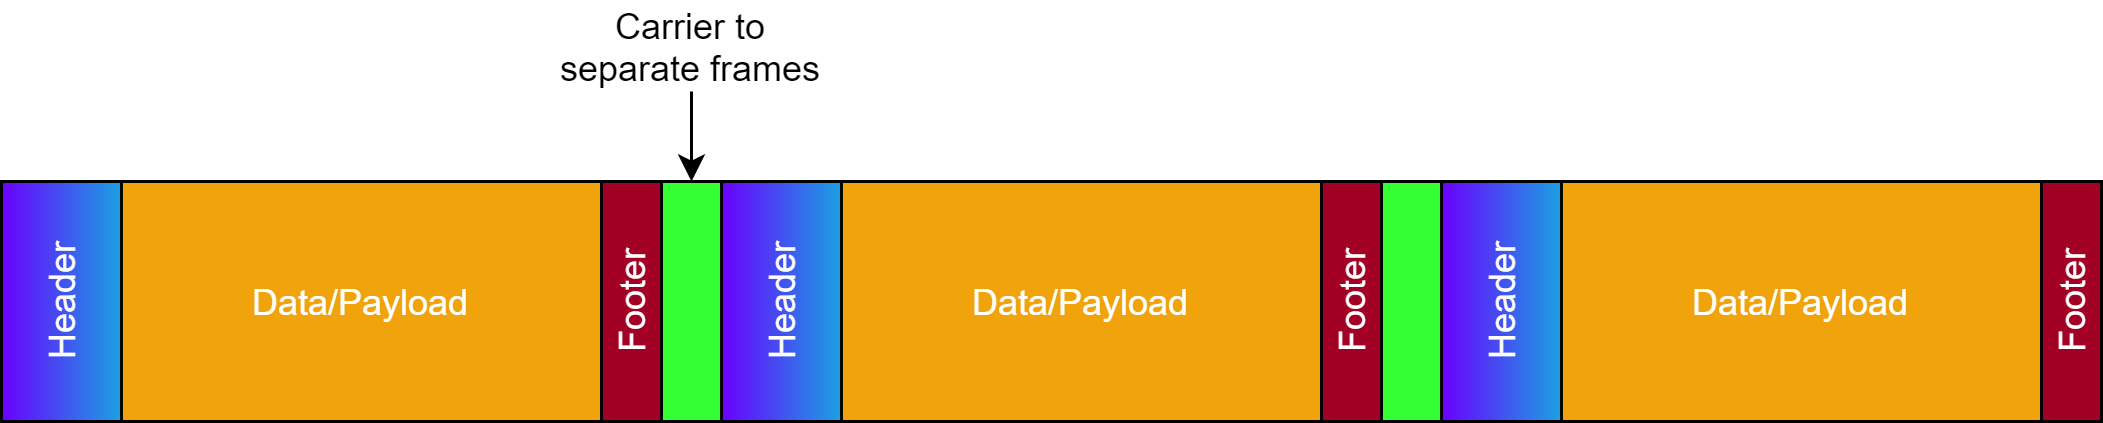
\includegraphics[width=0.7\textwidth]{data_link_layer/images/frame bursting}\end{center}
}

\subsection{Channel Back-Off}
\begin{center}
    \begin{tabular}{l p{0.8\textwidth}}
        \keyword{1-persistent}   & (Aggressive algorithm) Continually check channel. Transmit as soon as the channel is free. Used by \keyword{Ethernet}.            \\
        \keyword{Non-persistent} & (Non-Aggressive algorithm) Check channel, if idle translate immediately, else wait a random period of time before checking again. \\
        \keyword{P-persistent}   & Continually check channel, if it is free then transmit with probability $p$ (between 1 and Non persistent).                       \\
    \end{tabular}
\end{center}
\subsubsection{Binary Exponential Back-Off}
When network load is high (lots of contention for channels) \keyword{binary exponential back-off} is used.
\compitem{
    \item Slot length is the minimum frame length.
    \item If a collision occurs in transmission, wait $0$ or $1$ slots before attempting again.
    \item After $c$ collisions, wait $0$ to $2^c - 1$ slots (up to limit of $1023$ slots / $10$ collisions)
}
High contention $\to$ lots of collisions $\to$ \keyword{binary exponential back-off} $\to$ re-transmission attempts spread out $\to$ fewer collisions

\subsection{Medium Access through Token Passing}
There is a single token, stations can only transmit when they have the token.
\compitem{
    \item Token transfered with special token frame.
    \item If a station has the token but no frame to send, pass token on immediately.
    \item If a station has the token and a frame to send. It sets a timer and transmits until the timer expires or there is no more data to send. Then passes token.
}
\keyword{Ethernet} became much more popular, and hence has become the standard.

\subsection{Avoiding Wired Collisions using Switches}
A switch can remove the possibility of collisions by buffering frames and retransmitting when a channel becomes available.
\compitem{
    \item Each channel (ethernet cable) has only two stations (host and the switch)
    \item Hosts can transmit simultaneously, switch recieves and forwards frames.
    \item Maximum cable length determined by signal strength.
    \item \keyword{Switches} act as \keyword{repeaters}, refreshing the signal to pass it further.
}

\section{Address Resolution Protocol (ARP)}
In order to communicate outside of a network, an \keyword{IP Address} is required.
\compitem{
    \item Switches are in the \keyword{data-link layer} and do not use \keyword{IP Addresses} (in \keyword{network layer})
    \item \keyword{IP Address} can be set statically (fixed \keyword{IP}, set manually) or dynamically (assigned to your \keyword{NIC}, e.g by \ \keyword{DHCP} service).
    \item \keyword{IP Addresses} specify hosts on the \keyword{internet}, it does not have to be translated when passing through a router (but can, e.g \keyword{NAT}).
    \item \keyword{MAC Addresses} specify hosts communicating on the same network/subnetwork. Typically do not change when passing through routers (as packets).
}
In order to translate \keyword{IP Addresses} to \keyword{MAC Addresses} and vice-versa we use \keyword{ARP}.
\subsubsection{ARP Communication}
\begin{enumerate}
    \bullpara{Router}{Ask all hosts if they have a given \keyword{IP Address}
        \\ Places \keyword{ARP Message} query in a Data-link frame and broadcasts.
    }
    \bullpara{Host}{Checks if it has the requested address, if so sends a reply with its \keyword{MAC Address}}
    \bullpara{Router}{Recieves \keyword{ARP Message} with \keyword{MAC Address} and uses it.
        \\ Will forward \keyword{IP Datagrams} (encapsulated in a \keyword{Data-Link Frame}).
        \\ Usually also cache the \keyword{IP} $\to$ \keyword{MAC} translation
    }
\end{enumerate}
Some optimisations include caching recent \keyword{ARP Message} replies, or having all hosts broadcast their \keyword{IP} and \keyword{MAC Address} on boot/connection (as a network policy).

\begin{center}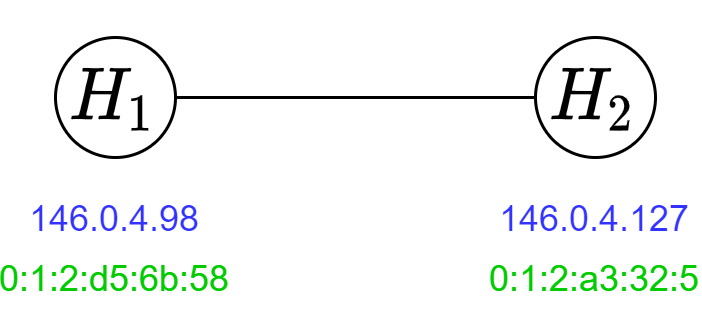
\includegraphics[width=0.4\textwidth]{data_link_layer/images/arp example}\end{center}
\begin{center}
    \begin{tabular}{l l l | l l l | l }
        \multicolumn{3}{c}{\textbf{Source}} & \multicolumn{3}{c}{\textbf{Destination}} & \multirow{2}{*}{\textbf{Message}}                                                                        \\
        \textbf{Host}                       & \textbf{IP}                              & \textbf{MAC}                      & \textbf{Host} & \textbf{IP}   & \textbf{MAC}        &                \\
        $H_2$                               & $146.0.4.127$                            & $0:1:2:a3:32:5$                   & All           & $146.0.4.98$  & $ff:ff:ff:ff:ff:ff$ & ARP Req        \\
        $H_1$                               & $146.0.4.98$                             & $0:1:2:d5:6b:58$                  & $H_2$         & $146.0.4.127$ & $0:1:2:a3:32:5$     & ARP Resp       \\
        $H_2$                               & $146.0.4.127$                            & $0:1:2:a3:32:5$                   & $H_1$         & $146.0.4.98$  & $0:1:2:d5:6b:58$    & ICMP Echo Req  \\
        $H_1$                               & $146.0.4.98$                             & $0:1:2:d5:6b:58$                  & $H_2$         & $146.0.4.127$ & $0:1:2:a3:32:5$     & ICMP Echo Resp \\
        $H_2$                               & $146.0.4.127$                            & $0:1:2:a3:32:5$                   & $H_1$         & $146.0.4.98$  & $0:1:2:d5:6b:58$    & ICMP Echo Req  \\
        $H_1$                               & $146.0.4.98$                             & $0:1:2:d5:6b:58$                  & $H_2$         & $146.0.4.127$ & $0:1:2:a3:32:5$     & ICMP Echo Resp \\
    \end{tabular}
\end{center}
\codelist{bash}{data_link_layer/code/arp_chain.txt}

\sidenote{ARP cache poisoning}{
    Malicious users can send spoof \keyword{ARP Messages} to attempt to associate their \keyword{MAC Address} with a victim's \keyword{IP Address} (thus receiving their \keyword{IP Datagrams})
    \\
    \\ This is covered in detail on the \href{https://en.wikipedia.org/wiki/ARP_spoofing}{wikipedia page}.
}
